\documentclass[xcolor=dvipsnames,10pt,aspectratio=169]{beamer}
%\usetheme[hideallsubsections]{Hannover}
\usetheme[width=1.9cm]{Hannover} % plenty of themes to pick from
\usefonttheme[onlymath]{serif}
\graphicspath{{../../images/}}
\usepackage[utf8]{inputenc}
\usepackage[T1]{fontenc}
\usepackage{amsmath}
\usepackage{amsfonts}
\usepackage{amssymb}
\usepackage{braket}
\usepackage{bm}
\usepackage{textpos}
\usepackage{multicol}
\usepackage{graphicx,hyperref,url}
\usepackage{tikz}
\usepackage{verbatim}
\usepackage{pgfplots}
\usetikzlibrary{arrows,shapes}
\usecolortheme{crane} % plenty of color themes to pick from
\useinnertheme{rectangles}

\definecolor{UBCgreen}{RGB}{30, 77, 43} % UBC Blue (primary)
\definecolor{UBCgold}{RGB}{200, 195, 114} % UBC Grey (secondary)

\setbeamercolor{palette primary}{bg=UBCgreen,fg=white}
\setbeamercolor{palette secondary}{bg=UBCgreen,fg=white}
\setbeamercolor{palette tertiary}{bg=UBCgreen,fg=white}
\setbeamercolor{palette quaternary}{bg=UBCgreen,fg=white}
\setbeamercolor{palette sidebar primary}{fg=black,bg=UBCgold}
\setbeamercolor{palette sidebar secondary}{fg=black,bg=UBCgold}
\setbeamercolor{palette sidebar tertiary}{fg=black,bg=UBCgold}
\setbeamercolor{palette sidebar quaternary}{fg=black,bg=UBCgold}
\setbeamercolor{structure}{fg=UBCgreen} % itemize, enumerate, etc
\setbeamercolor{section in toc}{fg=UBCgreen} % TOC sections
\setbeamercolor{subsection in head/foot}{bg=UBCgold,fg=white}
\setbeamercolor{section in sidebar}{fg=UBCgreen}
\setbeamercolor{section in sidebar}{fg=UBCgreen}
\setbeamerfont{section in sidebar}{size=\small}
\setbeamerfont{title in sidebar}{size=\tiny}
\setbeamerfont{author in sidebar}{size=\tiny}
\setbeamertemplate{page number in head/foot}[appendixframenumber]
\setbeamertemplate{navigation symbols}{\footnotesize\usebeamertemplate{page number in head/foot}}
\setbeamertemplate{frametitle}[default][left,colsep=-4bp,rounded=false]
\setbeamertemplate{section in toc}[bullets]

\addtobeamertemplate{title page}{}{%
    \begin{textblock*}{100mm}(0.445\textwidth,-22.4em)
      
\includegraphics[width=1.5cm]{./figures/CSU-Ram-357-617.png}
    \end{textblock*}
    \begin{textblock*}{75em}(-1.0em,-12em)
      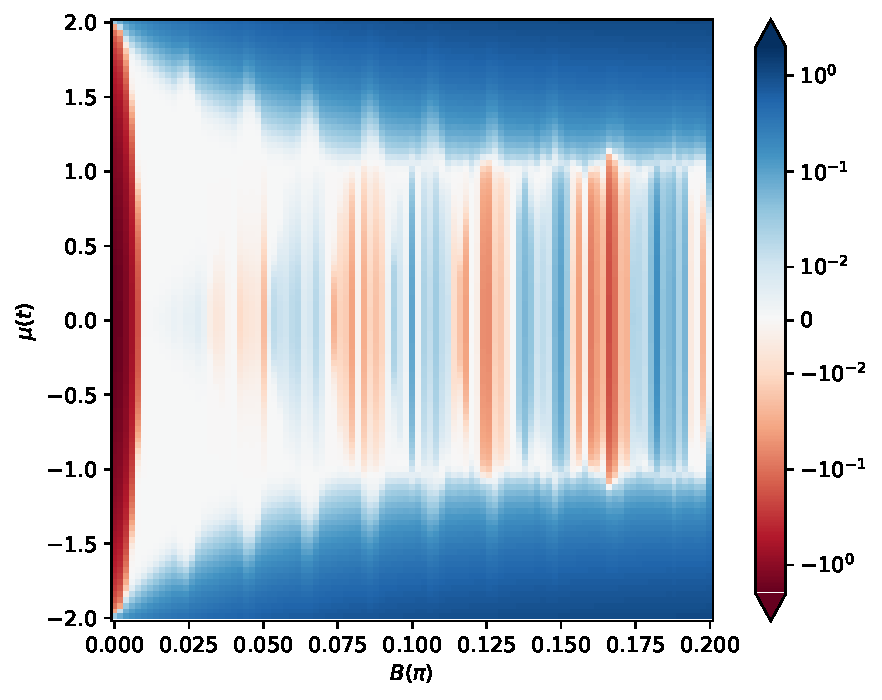
\includegraphics[width=0.18\textwidth]{./figures/linear-chain-majorana-number-full-range.pdf}
    \end{textblock*}
    \begin{textblock*}{75em}(24.0em,-12em)
      \includegraphics[width=0.19\textwidth]{../../../research-code/mf-quantum-logic-gate-scripts/data/figures/linear-vector-potential/nr-25/w-3/mu-p0_0000/En00-B-0_1029.pdf}
    \end{textblock*}
    \begin{textblock*}{100em}(-4.8em,16em)
      \tiny Powered by \LaTeX
    \end{textblock*}
}

\addtobeamertemplate{frametitle}{}{%
    \begin{textblock*}{100mm}(0.95\textwidth,-0.95cm)
      
\includegraphics[width=0.925cm]{./figures/CSU-Ram-357-617.png}
    \end{textblock*}
}
\makeatletter
\setbeamertemplate{sidebar canvas \beamer@sidebarside}%
                  [vertical shading][top=UBCgold,bottom=UBCgold]
\makeatother

%\addtobeamertemplate{sidebar left}{}{
%  \hspace{0.3cm}
%  \vspace{0.2cm}
%  
\includegraphics[align = l, width = 1cm]{./figures/CSU-Ram-357-617.png}
%}

%\setbeamertemplate{section in toc}{\hspace*{0em}\inserttocsection}
%\setbeamertemplate{subsection in toc}{\hspace*{2em}\inserttocsubsection}

\let\oldhat\hat
\renewcommand{\hat}[1]{\oldhat{\mathbf{#1}}}
\renewcommand{\vec}[1]{\mathbf{#1}}

\newcommand{\ham}{\mathcal{H}}
\newcommand{\ke}{k_{\epsilon}}
\newcommand{\kpm}{k_{\pm}}
\newcommand{\sx}{\sigma_x}
\newcommand{\sy}{\sigma_y}
\newcommand{\sz}{\sigma_z}
\newcommand{\so}{\sigma_0}
\newcommand{\cc}{c^{\dagger}}
\newcommand{\de}{\Delta}

\newcommand{\TT}{Searching for Majorana Corner Modes in Triangular Superconducting Islands}
\newcommand{\ST}{Searching for Majorana corner modes in triangular superconducting islands}
\newcommand{\BD}{Background}
\newcommand{\MO}{Motivation}
\newcommand{\PW}{Previous Work}
\newcommand{\FO}{Formulation}
\newcommand{\RE}{Results}
\newcommand{\CO}{Summary}

\title[\ST]{\TT}
\subtitle{}
\author[Aidan Winblad]{Aidan Winblad \small \and\\ Hua Chen}
\institute{Department of Physics \and\\ Colorado State University}
\date{\small October 26, 2022}

\begin{document}

  \begin{frame}
  \titlepage
  \end{frame}

  \begin{frame}
  \frametitle{Outline}
    \begin{itemize}
      \item \BD:
        \begin{itemize}
          \footnotesize
          \item Majorana fermions in particle physics and condensed matter
          \item Quantum information storage
        \end{itemize}
      \item \MO:
        \begin{itemize}
          \footnotesize
          \item Braiding in a 2D \textit{p}-wave SC
          \item T-junctions
          \item Triangular structures for braiding
        \end{itemize}
      \item \FO: Two Approaches
        \begin{itemize}
          \footnotesize
          \item Topological phase diagram for linear vector potential on Kitaev chain
          \item[] Bulk-edge correspondence for a double chain model
          \item Vector potential on a triangular island in the Kitaev limit
        \end{itemize}
      \item \RE:
        \begin{itemize}
          \footnotesize
          \item MCMs on 3 triangular structures
        \end{itemize}
      \item \CO
        \begin{itemize}
          \footnotesize
          \item Conclusions
          \item Additional projects
        \end{itemize}
    \end{itemize}
  \end{frame}

  \section{\BD}

  \begin{frame}{\BD: MFs in Particle Physics}
    \begin{multicols}{2}
      \centering
      \begin{tikzpicture}
        \node[inner sep=0pt] (figure) at (-1,0)
        {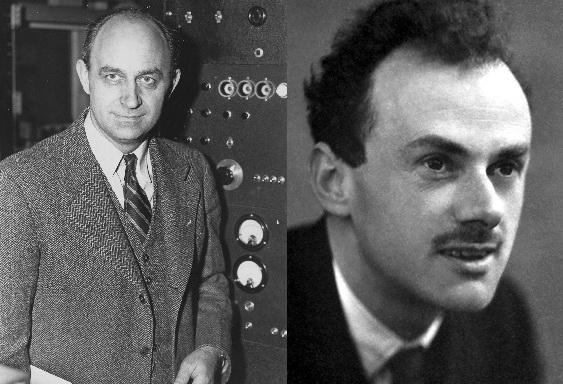
\includegraphics[width=0.4\textwidth]{./figures/Fermi-Dirac.jpg}};
        \node[inner sep=0pt] (Fermi) at (-2.35,-2.0) {\small Enrico Fermi};
        \node[inner sep=0pt] (Dirac) at (0.35,-2.0) {\small Paul Dirac};
      \end{tikzpicture}

      \vspace{1.0pt}

      \centering
      \begin{tikzpicture}
        \node[inner sep=0pt] (figure) at (0,0)
        {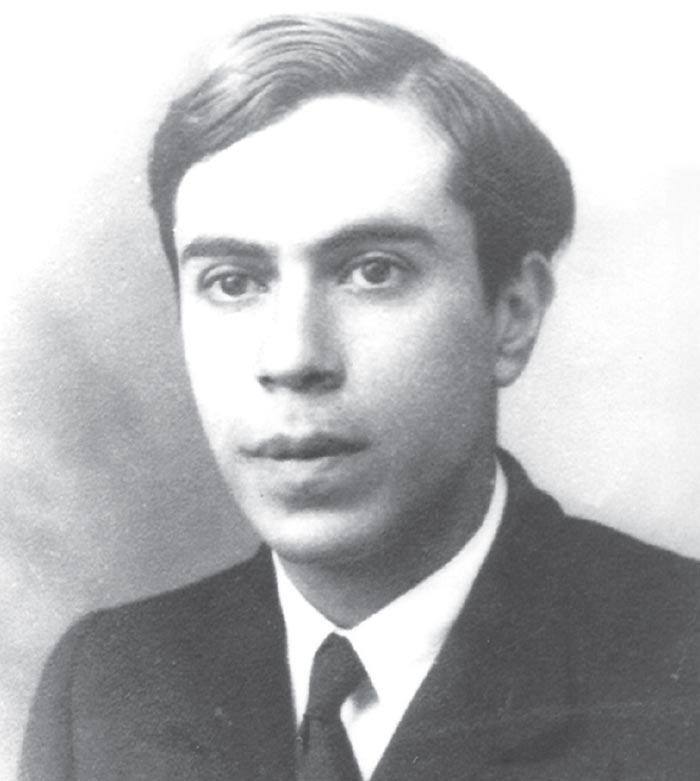
\includegraphics[width=0.18\textwidth]{./figures/Ettore_Majorana.jpg}};
        \node[inner sep=0pt] (Enrico) at (0,-1.65) {\small Ettore Majorana}
      \end{tikzpicture}

      \begin{itemize}
        \setlength\itemsep{0pt}
        \small
        \item Fermions
          \begin{itemize}
            \item Half-odd-integer spin
            \item Fermi-Dirac statistics
            \item Weyl fermions are massless
          \end{itemize}
      \end{itemize}
      \begin{itemize}
        \setlength\itemsep{0pt}
        \small
        \item  Dirac Fermions
        \begin{itemize}
          \item Particle $\neq$ Antiparticle : $c \neq c^{\dagger}$
          \item Charged
        \end{itemize}
      \end{itemize}

      \begin{itemize}
        \setlength\itemsep{0pt}
        \small
        \item Majorana Fermions
        \begin{itemize}
            \item Particle $=$ Antiparticle : $c = c^{\dagger}$
            \item Neutral
            \item Neutrino? Dark Matter?
        \end{itemize}
      \end{itemize}

    \end{multicols}

  \end{frame}

  \begin{frame}{\BD: MFs in Particle Physics}
    \begin{multicols}{2}
      \centering
      \begin{tikzpicture}
        \node[inner sep=0pt] (figure) at (0,0)
        {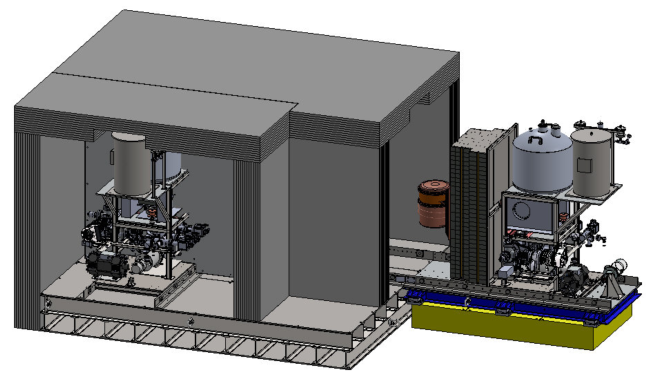
\includegraphics[width=0.5\textwidth]{./figures/majorana-experiment.png}};
        \node[inner sep=0pt] (reference) at (0,-2.1) {\small MAJORANA project:};
        \node[inner sep=0pt] (reference) at (0,-2.5) {\small neutrinoless double beta (0$\nu\beta\beta$) decay};
      \end{tikzpicture}

      \begin{itemize}
          \item Are neutrinos Majorana fermions?
          \item If yes, standard model needs revision
          \item Negative results for Majorana particles
      \end{itemize}

    \end{multicols}
  \end{frame}

  \begin{frame}{\BD: MFs in Condensed Matter}
    \begin{multicols}{2}
      \begin{itemize}
        \item Superconductors
          \begin{itemize}
            \item Cooper pairs
            \begin{itemize}
              \item Electron-phonon interaction pairs two electrons with opposite spin and momenta.
            \end{itemize}
            \item Bogoliubov quasiparticles
            \begin{itemize}
              \item Excitation from ground state, pairs an electron to a hole.
              \item[] \[ H_{BdG} = \begin{bmatrix} \epsilon(k) & \de(k) \\ \de^\ast(k) & -\epsilon(-k) \end{bmatrix} \]
              \item Zero-energy excitations may be Majorana fermions.
              \item If so, they come in pairs.
            \end{itemize}
          \end{itemize}
      \end{itemize}
      \vspace{30mm}

      \begin{tikzpicture}
        \node[inner sep=0pt] (figure) at (0,0)
        {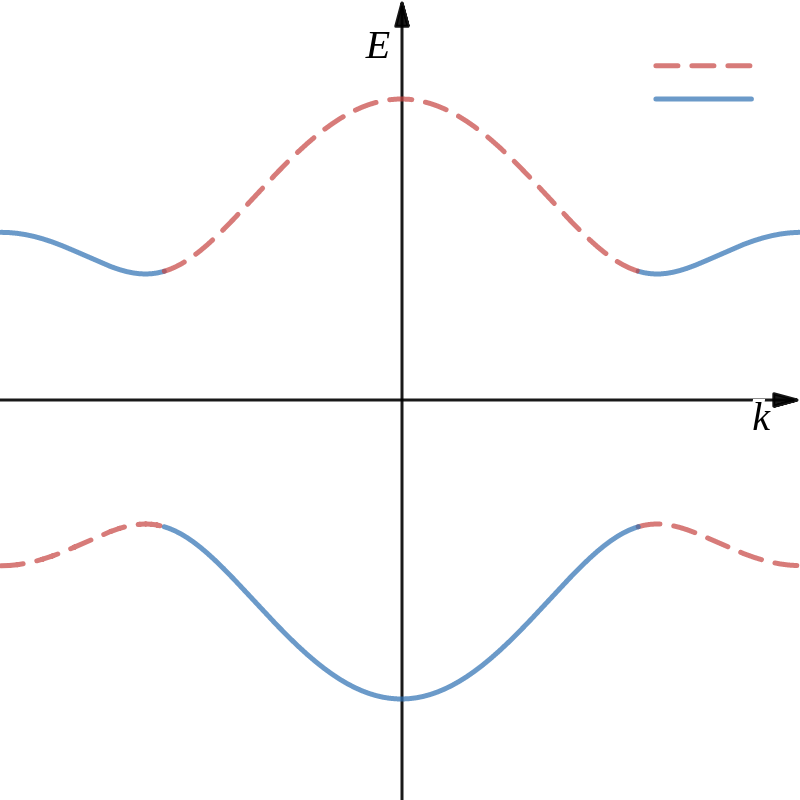
\includegraphics[width=0.45\textwidth]{./figures/electron-holes-dispersion.png}};
        \node[inner sep=0pt] (holes) at (1.4,2.5) {\small holes};
        \node[inner sep=0pt] (electrons) at (1.15,2.25) {\small electrons};
      \end{tikzpicture}

    \end{multicols}

  \end{frame}

  \begin{frame}{\BD: MFs in Condensed Matter}
    \begin{tikzpicture}
      \node[inner sep=0pt] (figure) at (0,0)
      {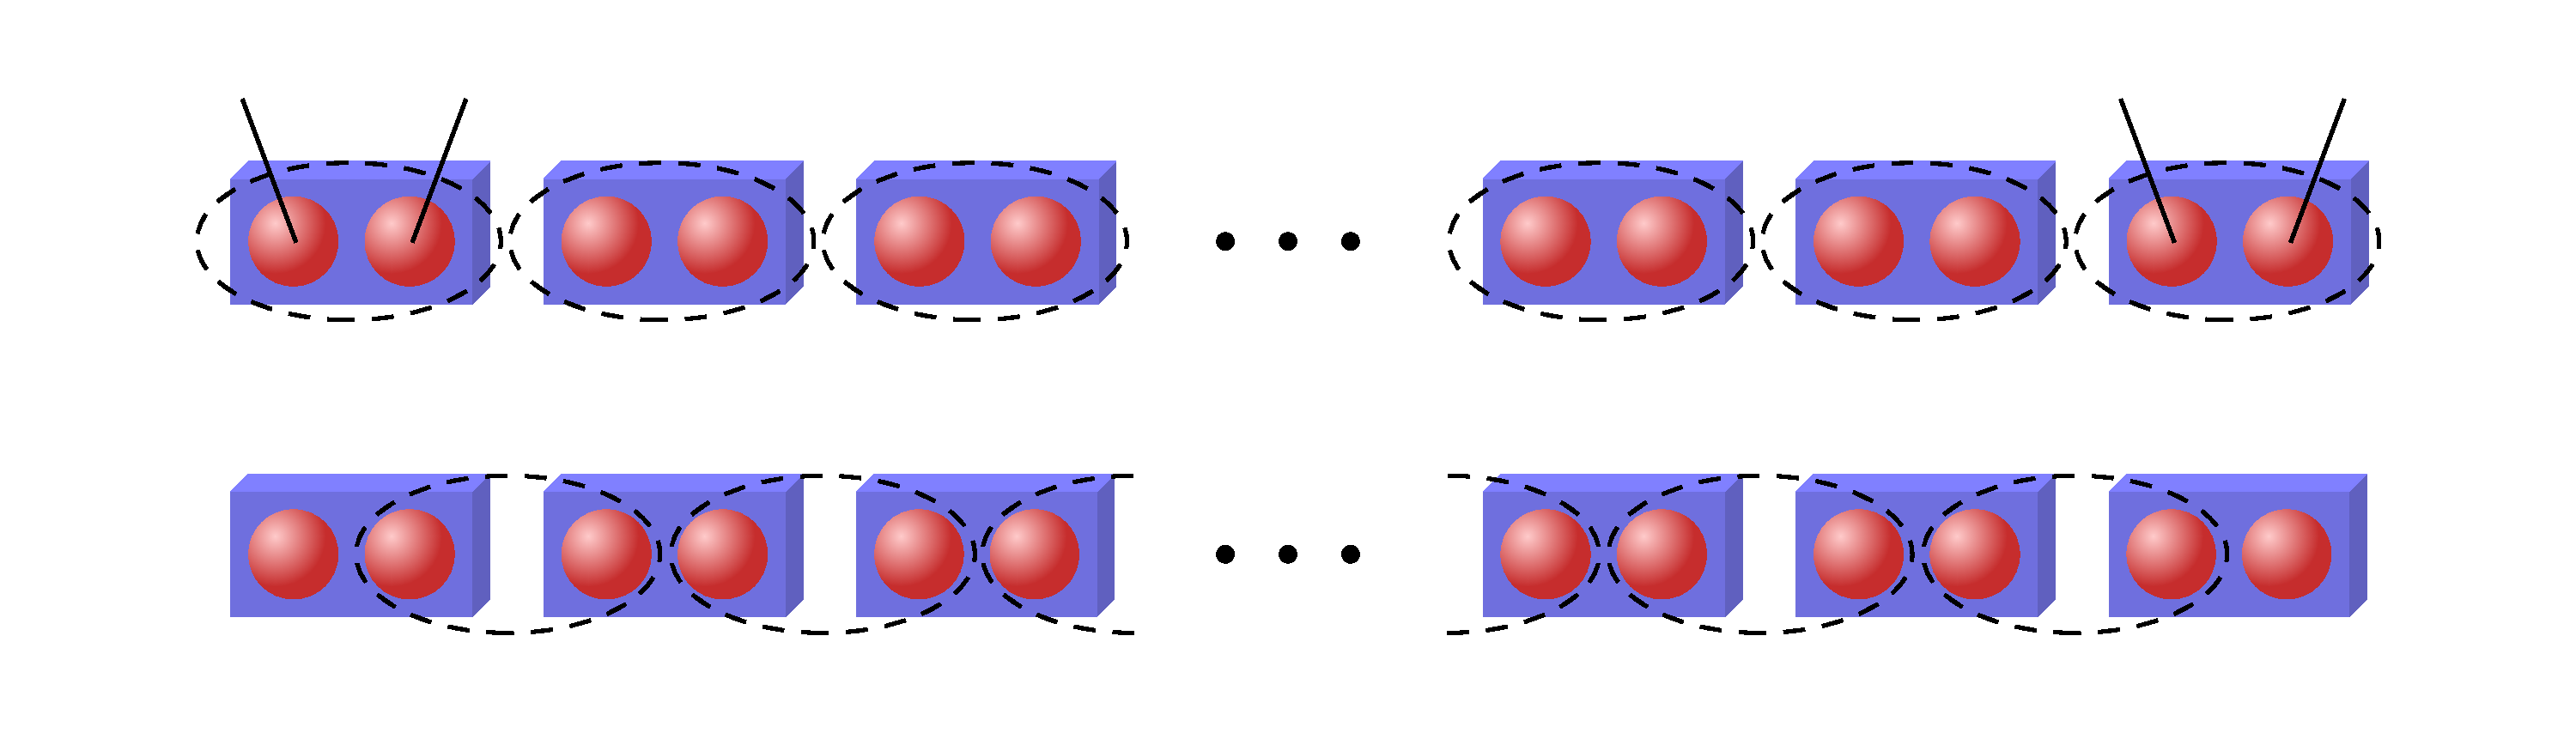
\includegraphics[width=\textwidth]{./figures/Kitaev Chain.pdf}};
      \node[inner sep=0pt] (a1) at (-4.7,1.6) {\small $a_1$\quad\quad\quad$b_1$};
      \node[inner sep=0pt] (aN) at (4.9,1.6) {\small $a_N$\quad\quad\ \ $b_N$};
      \node[inner sep=0pt] (c1) at (-4.75,0) {\small $c_1$};
      \node[inner sep=0pt] (cN) at (4.9,0) {\small $c_N$};
      \node[inner sep=0pt] (cc1) at (-3.9,-1.6) {\small $\tilde{c}_1$};
      \node[inner sep=0pt] (ccN) at (4.3,-1.6) {\small $\tilde{c}_{N-1}$};
      \node[inner sep=0pt] (reference) at (0.0,-2.0) {\footnotesize Kitaev, Phys, Uspekhi \textbf{44}, 131 (2001)};
    \end{tikzpicture}

    \vspace{20pt}
    Complex fermion in Majorana fermion basis
    \begin{equation}
      c_j = \dfrac{1}{2}(a_j + i b_j).
    \end{equation}

  \end{frame}

  \begin{frame}{\BD: MFs in Condensed Matter}
    Hamiltonian for a 1D tight-binding chain with spinless \textit{p}-wave superconductivity
    \begin{equation}
      \ham_{chain} = -\mu\sum_j^N \cc_j c_j -\sum_j^{N-1} t \cc_j c_{j+1} + |\de| c_j c_{j+1} + h.c.
    \end{equation}
    Hamiltonian in Majorana fermion basis
    \begin{equation}
      \ham_{chain} = \dfrac{i}{2} \sum_j -\mu a_j b_j + (t+|\de|) b_j a_{j+1} + (-t+|\de|) a_j b_{j+1}.
    \end{equation}
    $t=|\de|=0$ and $\mu<0$, trivial phase
    \begin{equation}
      \ham = -\dfrac{i\mu}{2} \sum_j a_j b_j.
    \end{equation}
    $t=|\de|>0$ and $\mu=0$, non-trivial (topological) phase
    \begin{equation}
      \ham = it \sum_j b_j a_{j+1}.
    \end{equation}

  \end{frame}

  \begin{frame}{\BD: MFs in Condensed Matter}
    \begin{tikzpicture}
      \node[inner sep=0pt] (figure) at (0,0)
      {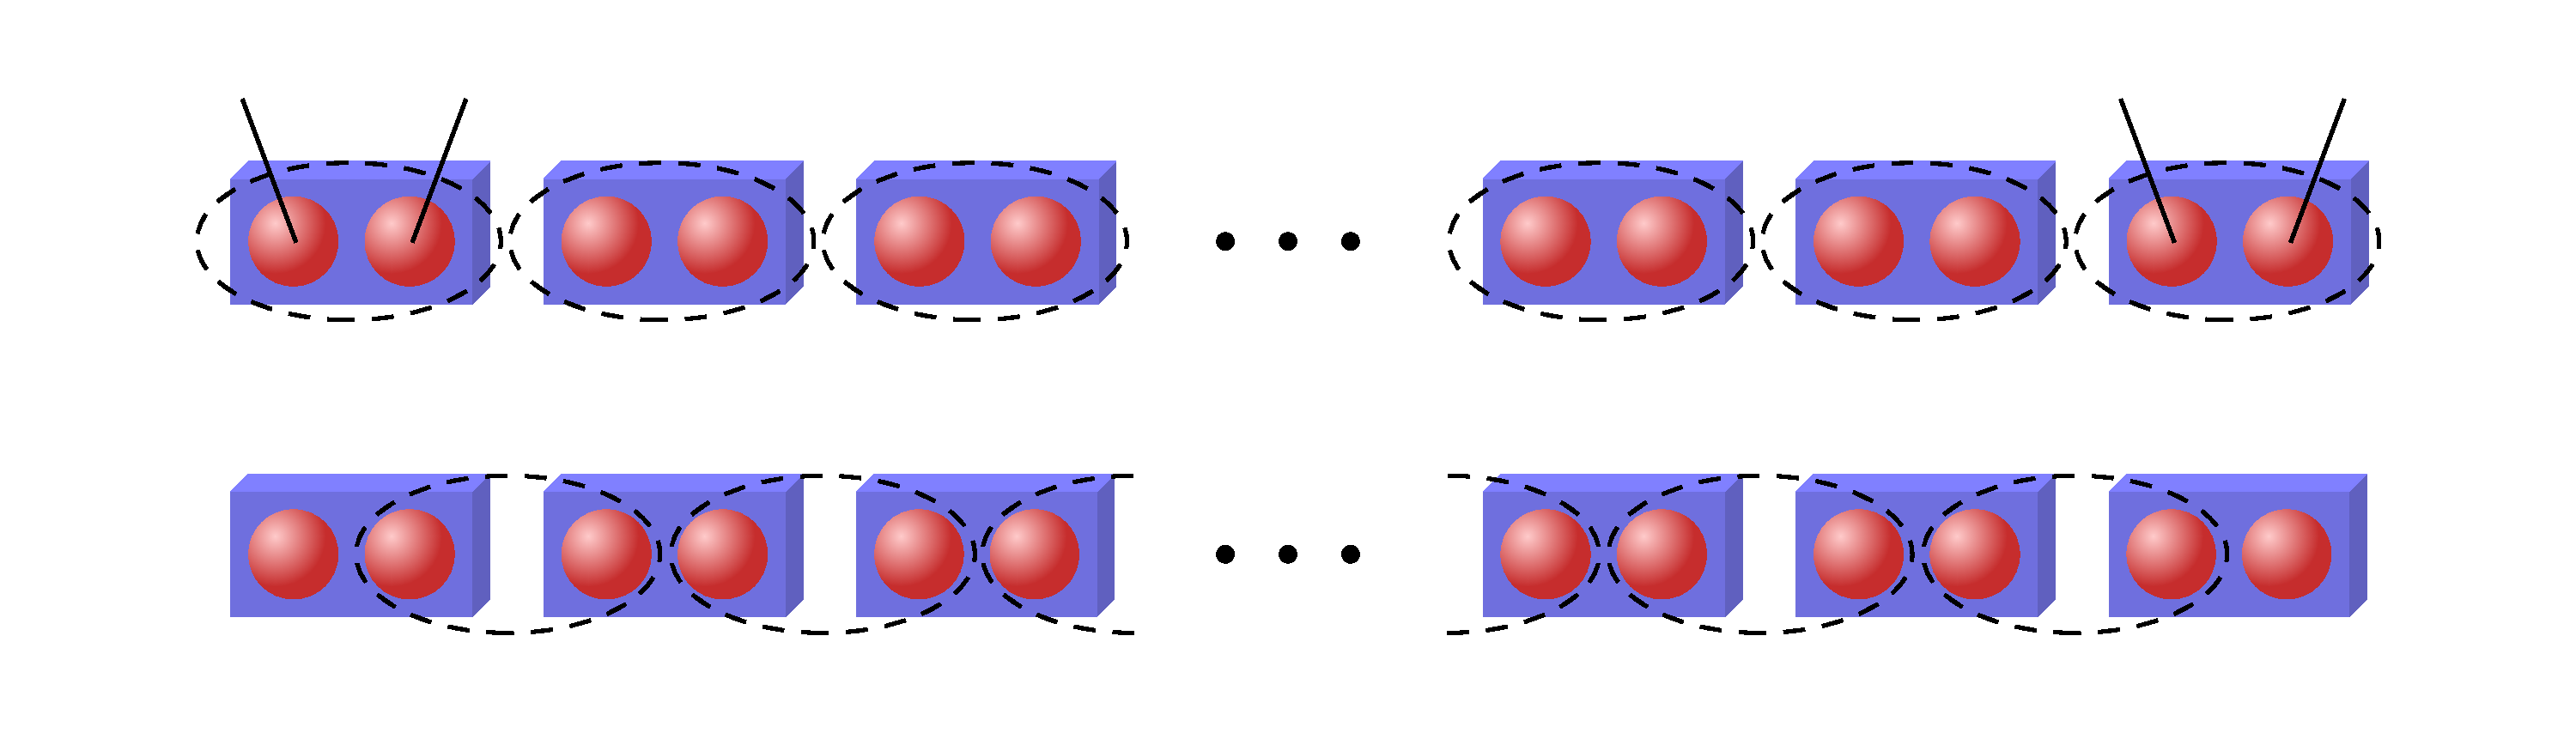
\includegraphics[width=\textwidth]{./figures/Kitaev Chain.pdf}};
      \node[inner sep=0pt] (a1) at (-4.7,1.6) {\small $a_1$\quad\quad\quad$b_1$};
      \node[inner sep=0pt] (aN) at (4.9,1.6) {\small $a_N$\quad\quad\ \ $b_N$};
      \node[inner sep=0pt] (c1) at (-4.75,0) {\small $c_1$};
      \node[inner sep=0pt] (cN) at (4.9,0) {\small $c_N$};
      \node[inner sep=0pt] (cc1) at (-3.9,-1.6) {\small $\tilde{c}_1$};
      \node[inner sep=0pt] (ccN) at (4.3,-1.6) {\small $\tilde{c}_{N-1}$};
      \node[inner sep=0pt] (reference) at (0.0,-2.0) {\footnotesize Kitaev, \textit{Phys. Uspekhi} \textbf{44}, 131 (2001)};
      \node[inner sep=0pt] (H1) at (0,1.5) {\small $\ham = \dfrac{-i\mu}{2} \sum_j a_j b_j$};
      \node[inner sep=0pt] (H1) at (0,-0.2) {\small $\ham = it \sum_j b_j a_{j+1}$};
      \node[inner sep=0pt] (trivial) at (-6.1,0.7) {\small trivial};
      \node[inner sep=0pt] (trivial) at (-6.3,-0.9) {\small non-trivial};
    \end{tikzpicture}

    Intersite fermion representation
    \begin{equation}
      \tilde{c}_j = \dfrac{1}{2}(a_{j+1} + i b_j).
    \end{equation}
    The highly non-local fermion state
    \begin{equation}
      f = \dfrac{1}{2}(a_{1} + i b_N),
    \end{equation}
    corresponds to zero energy. This is still true for $|\mu|< 2t$.
  \end{frame}

  \begin{frame}{\BD: MFs in Condensed Matter}
    \begin{multicols}{2}
      \centering
      \begin{tikzpicture}
        \node[inner sep=0pt] (figure) at (0,0)
        {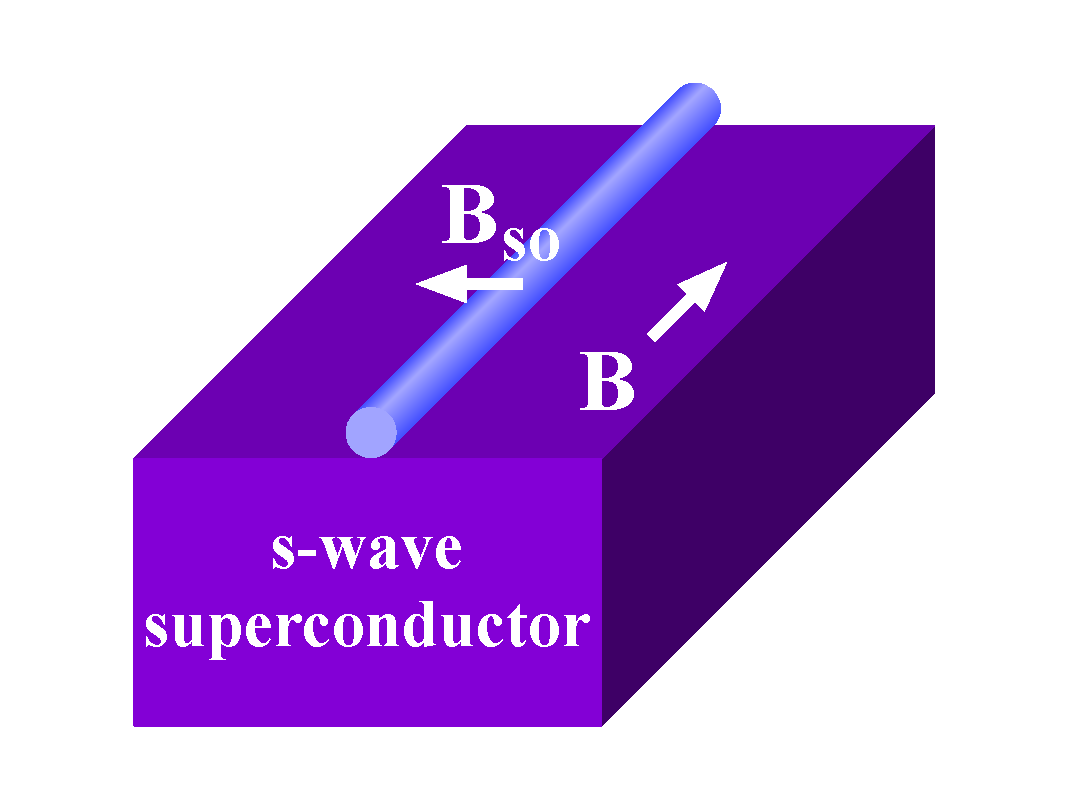
\includegraphics[width=0.35\textwidth]{./figures/swave-superconductor.pdf}};
      \end{tikzpicture}
      \begin{tikzpicture}
        \node[inner sep=0pt] (figure) at (0,0)
        {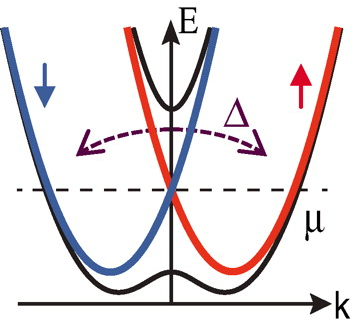
\includegraphics[width=0.30\textwidth]{./figures/Mourik-dispersion.jpeg}};
      \end{tikzpicture}
      \vspace{40pt}
      \begin{tikzpicture}
        \node[inner sep=0pt] (figure) at (0,0)
        {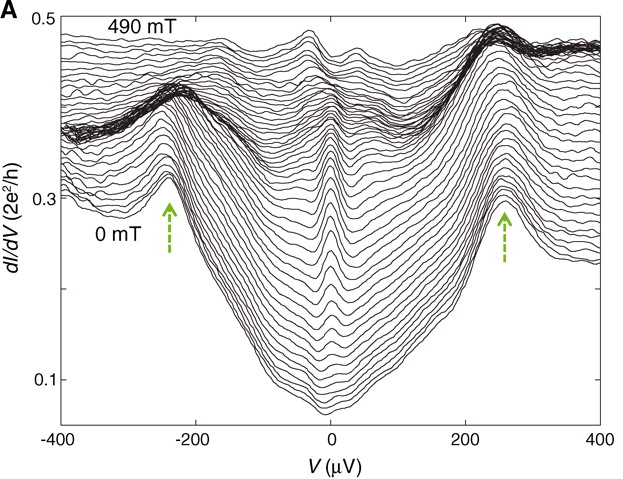
\includegraphics[width=0.50\textwidth]{./figures/Mourik-didv-curve.png}};
        \node[inner sep=0pt] (reference) at (0.25,-3) {\footnotesize Mourik et al., \textit{Science} \textbf{336}, 1003 (2012).};
      \end{tikzpicture}
    \end{multicols}
  \end{frame}

  \begin{frame}{\BD: MFs in Condensed Matter}
    \begin{tikzpicture}
      \node[inner sep=0pt] (figure) at (-4,0)
      {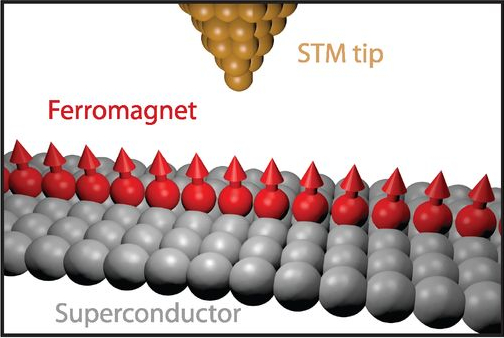
\includegraphics[width=0.5\textwidth]{./figures/Nadj-Perge-setup.png}};
      \node[inner sep=0pt] (figure) at (2.75,0)
      {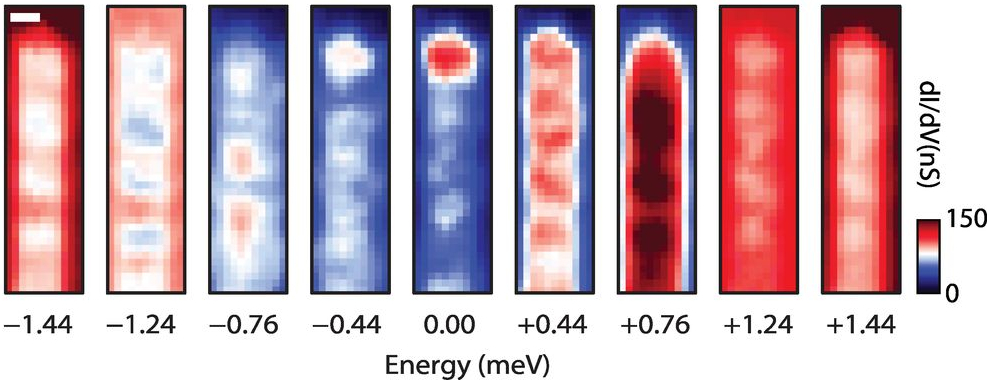
\includegraphics[width=0.5\textwidth]{./figures/Nadj-Perge-results.png}};
      \node[inner sep=0pt] (reference) at (2.75,-1.75) {\footnotesize Nadj-Perge et al., \textit{Science} \textbf{346}, 602 (2014).};
    \end{tikzpicture}
  \end{frame}

  \begin{frame}{\BD: MFs in Condensed Matter}
    \centering
    \begin{tikzpicture}
      \node[inner sep=0pt] (figure) at (0,0)
      {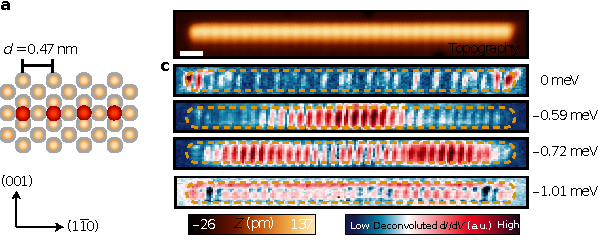
\includegraphics[width=\textwidth]{./figures/Schneider-results.pdf}};
      \node[inner sep=0pt] (reference) at (0,-3.00) {\footnotesize Mn atoms (red spheres) on top of superconducting Nb (brown spheres).};
      \node[inner sep=0pt] (reference) at (0,-3.40) {\footnotesize Schneider et al., \textit{Nature Nanotechnology} \textbf{17}, 384 (2022).};
    \end{tikzpicture}
  \end{frame}


  \section{\MO}

  \begin{frame}{\MO: Braiding in a 2D \textit{p}-wave SC}
    \begin{multicols}{2}
      \begin{figure}
        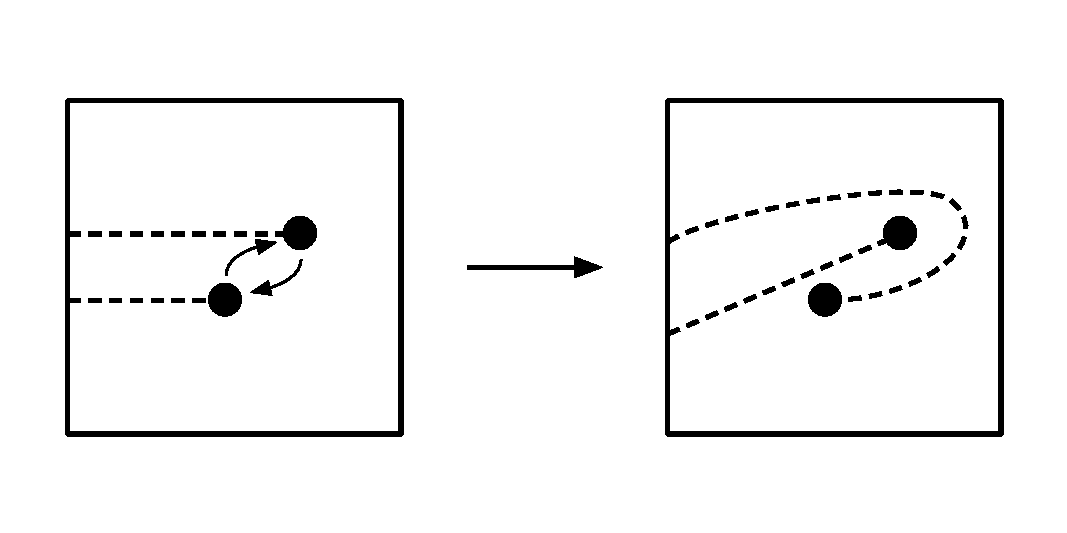
\includegraphics[width=0.5\textwidth]{./figures/pwave-braid.pdf}
      \end{figure}

      \begin{itemize}
          \item Interchanging two MFs:
          \begin{itemize}
            \item[] $\gamma_1 \rightarrow \gamma_2$ \\
            \item[] $\gamma_2 \rightarrow -\gamma_1$ \\
          \end{itemize}
          \item Exhibit Non-Abelian Statistics
          \item $a \ast b \neq b \ast a$
      \end{itemize}
      \begin{equation*}
      \end{equation*}
      \vspace{20pt}

      \centering
      \begin{tikzpicture}
        \node[inner sep=0pt] (figure) at (0,0)
        {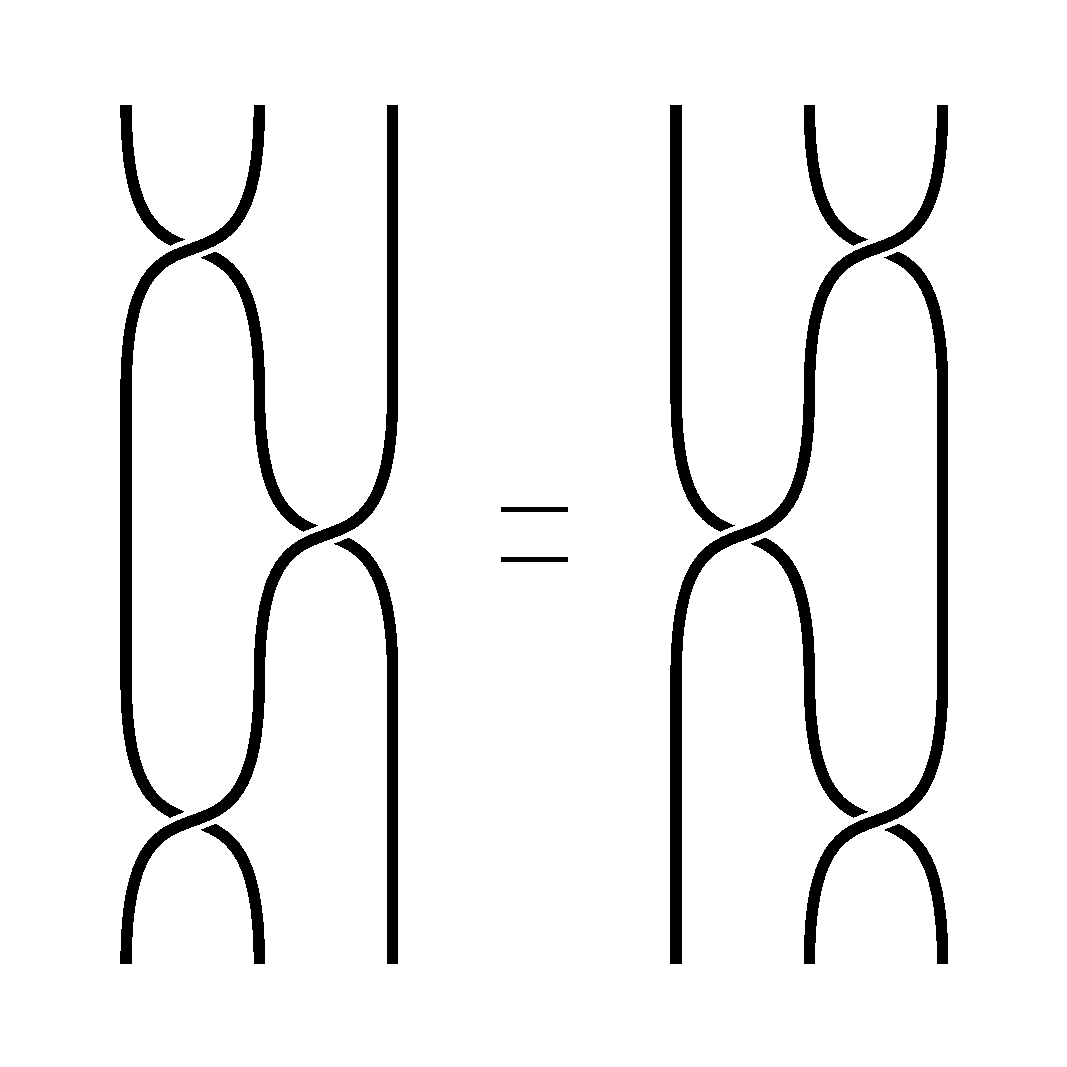
\includegraphics[width=0.45\textwidth]{./figures/braid.pdf}};
        \node[inner sep=0pt] (Ttl) at (-2.7,1.5) {\small $T_i$};
        \node[inner sep=0pt] (Ttr) at (2.7,1.5) {\small $T_{i+1}$};
        \node[inner sep=0pt] (Tml) at (-2.6,0.0) {\small $T_{i+1}$};
        \node[inner sep=0pt] (Tmr) at (2.5,0.0) {\small $T_i$};
        \node[inner sep=0pt] (Tbl) at (-2.7,-1.6) {\small $T_i$};
        \node[inner sep=0pt] (Tbr) at (2.7,-1.6) {\small $T_{i+1}$};
        \node[inner sep=0pt] (math) at (0, -3,0) {\small $T_i T_{i+1} T_i = T_{i+1} T_i T_{i+1}$};
        \node[inner sep=0pt] (reference) at (0,-3.5) {\footnotesize Ivanov, \textit{PRL} \textbf{86}, 268 (2001).};
      \end{tikzpicture}

    \end{multicols}
  \end{frame}

  \begin{frame}{\MO: T-junction as a Quantum Logic Gate}

    \begin{multicols}{3}
    \begin{figure}
      \begin{tikzpicture}
        \node[inner sep=0pt] (figure) at (0,0)
        {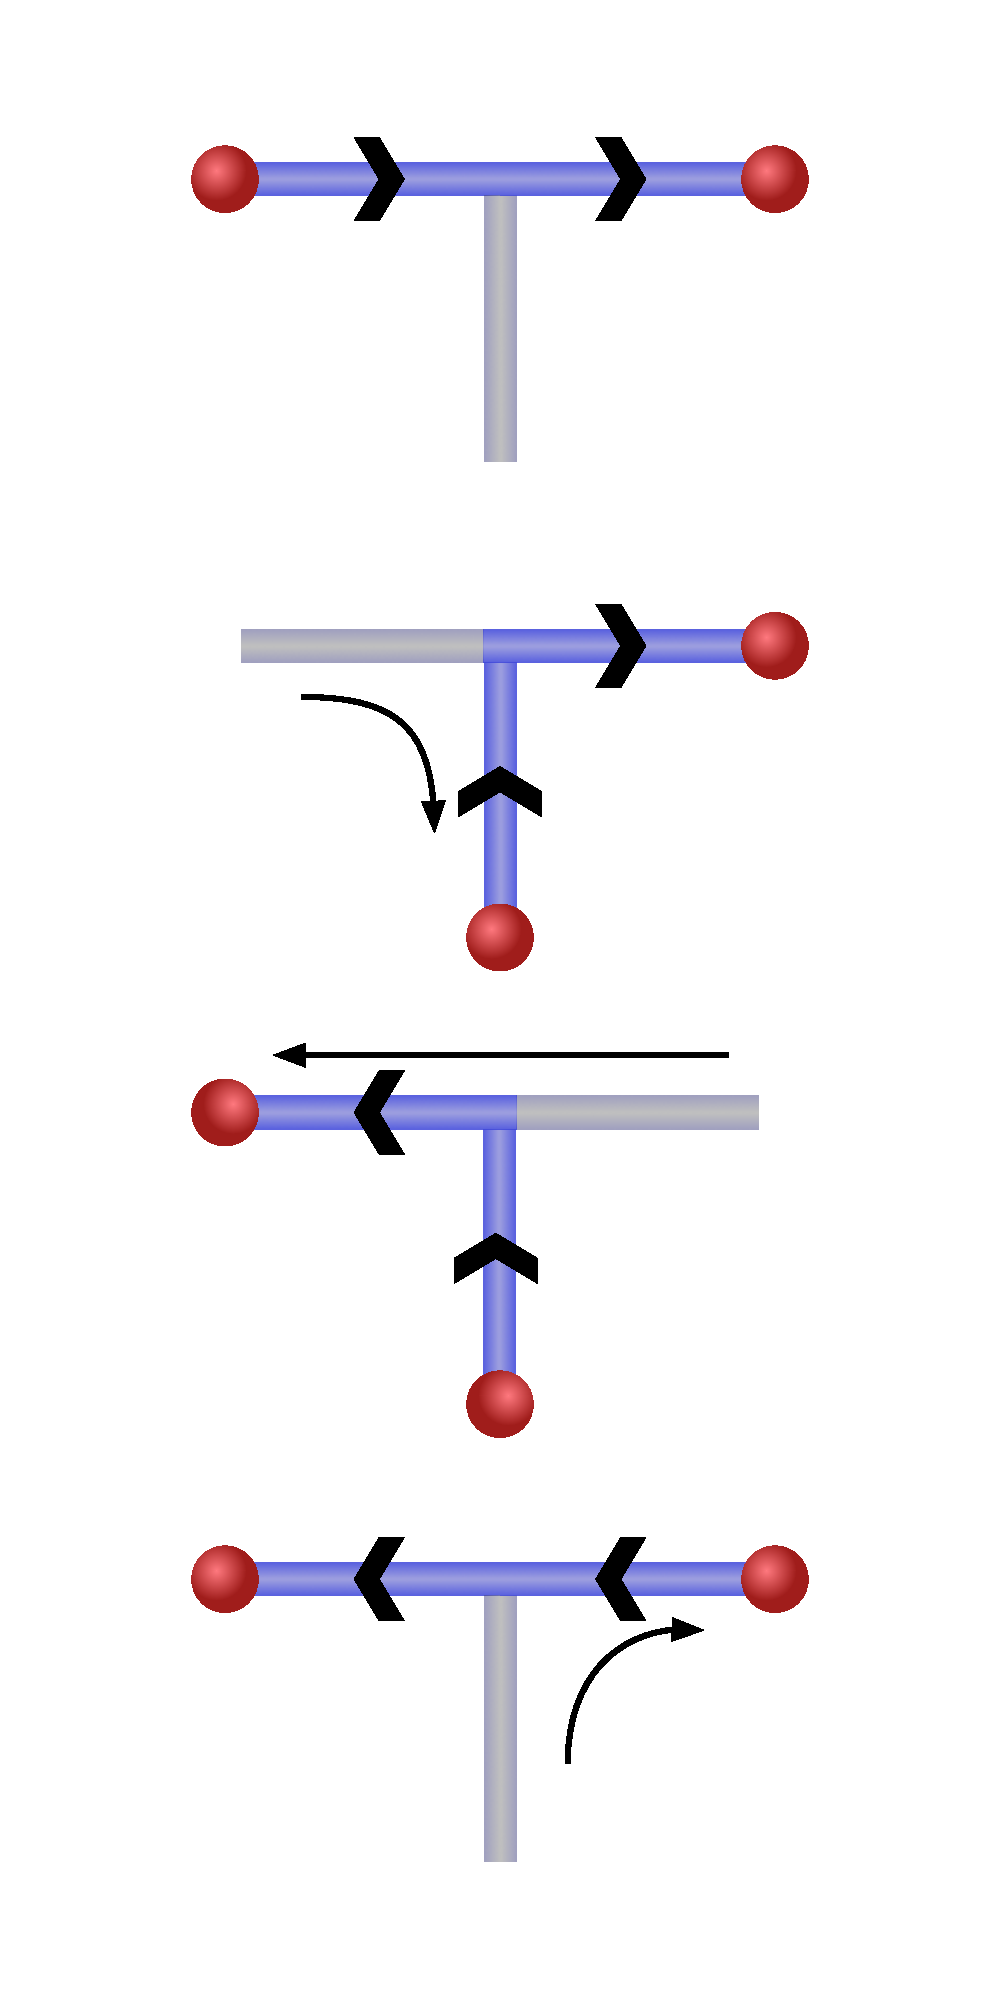
\includegraphics[width=0.30\textwidth]{./figures/t-junction.pdf}};
        \node[inner sep=0pt] (a1) at (-1.1,3.5) {\small $\gamma_1$};
        \node[inner sep=0pt] (a2) at (1.1,3.5) {\small $\gamma_2$};
        \node[inner sep=0pt] (b1) at (0.4,0.2) {\small $\gamma_1$};
        \node[inner sep=0pt] (b2) at (1.1,1.65) {\small $\gamma_2$};
        \node[inner sep=0pt] (c1) at (0.4,-1.65) {\small $\gamma_1$};
        \node[inner sep=0pt] (c2) at (-1.1,-0.15) {\small $\gamma_2$};
        \node[inner sep=0pt] (d1) at (1.1,-2.00) {\small $\gamma_1$};
        \node[inner sep=0pt] (d2) at (-1.1,-2.00) {\small $\gamma_2$};
        \end{tikzpicture}
      \end{figure}

      \begin{minipage}{0.67\textwidth}
      \small
      \begin{equation}
        \ham_T = -\mu \sum_j \cc_j c_j - \sum_j t \cc_j c_{j+1} + |\de| e^{i\phi} c_j c_{j+1} + h.c.
      \end{equation}
      \begin{equation}
        c_j = e^{-i(\phi/2)}(\gamma_{j+1,1} + i \gamma_{j,2})/2
      \end{equation}
      \begin{itemize}
        \footnotesize
        \item Take pairing term $|\de|e^{i\phi} c_j c_{j+1}$ such that the site indices:
        \item Increase moving $\rightarrow / \uparrow$ in the horizontal/vertical wires: $\phi=0$,
        \item Decrease moving $\leftarrow / \downarrow$ in the horizontal/vertical wires: $\phi=\pi$.
      \end{itemize}

      \centering
      \begin{tikzpicture}
        \node[inner sep=0pt] (figure) at (0,0)
        {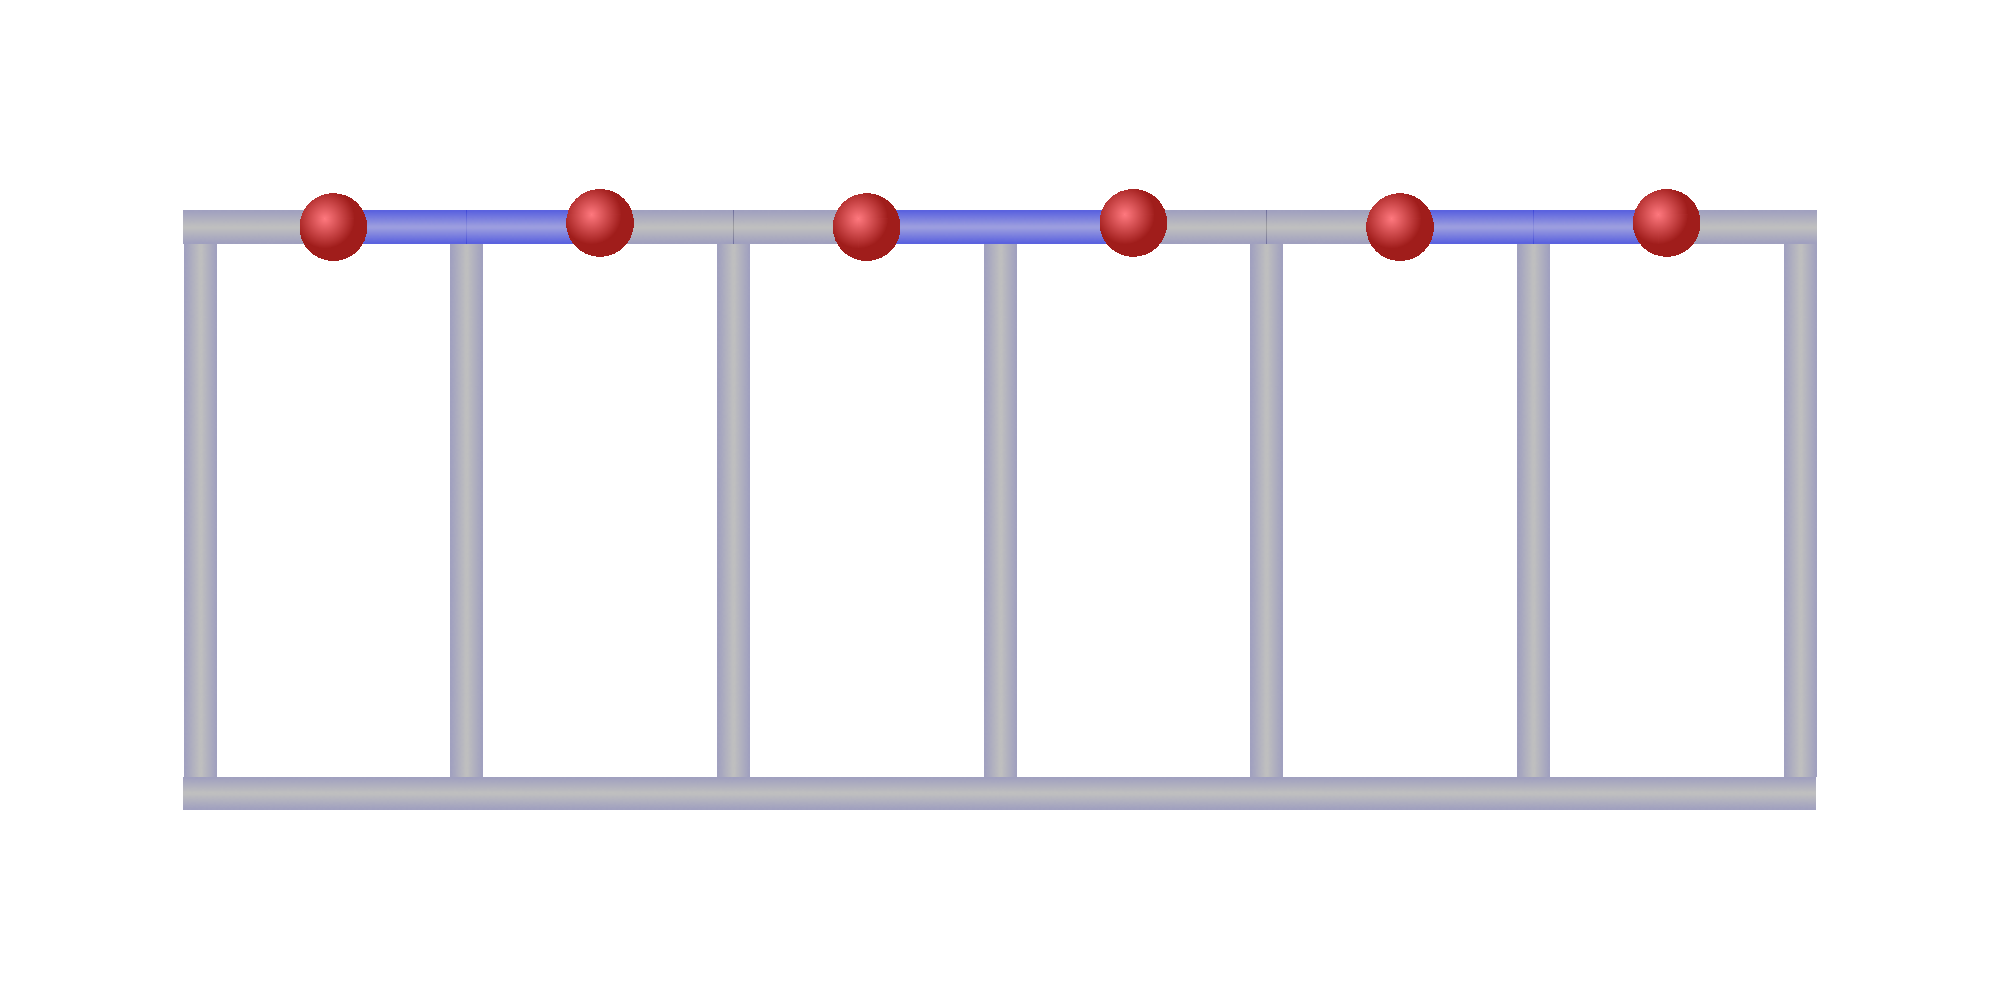
\includegraphics[width=0.8\textwidth]{./figures/t-junction-network.pdf}};
        \node[inner sep=0pt] (gamma1) at (-1.9,1.3) {\small $\gamma_1$ \quad\ \  $\gamma_2$};
        \node[inner sep=0pt] (gamma2) at (0.0,1.3) {\small $\gamma_3$ \quad\ \  $\gamma_4$};
        \node[inner sep=0pt] (gamma3) at (1.8,1.3) {\small $\gamma_5$ \quad\ \  $\gamma_6$};
        \node[inner sep=0pt] (reference) at (0,-1.5) {\small Alicea et al., \textit{Nature Phys.} \textbf{7}, 412 (2011)}
      \end{tikzpicture}
      \vspace{20cm}
      \end{minipage}

    \end{multicols}
  \end{frame}

  \begin{frame}
    \frametitle{\MO: Triangular Structures for Braiding}
    \begin{multicols}{2}

    \begin{itemize}
      \item Consider triangular islands, topologically similar to T-junctions.
      \item Islands of three-fold rotational symmetry occur naturally in epitaxial growth on close-packed metal surfaces.
      \item Make a smooth connection from 1D to 2D superconductors.
    \end{itemize}
    \newline

    \begin{figure}
      \begin{tikzpicture}
        \node[inner sep=0pt] (figure) at (0,0)
        {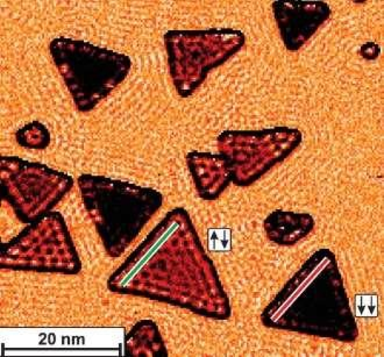
\includegraphics[width=0.4\textwidth]{./figures/triangular-islands.pdf}};
        \node[inner sep=0pt] (caption) at (0,-2.8) {\scriptsize Triangular Co islands on Cu(111).};
        \node[inner sep=0pt] (reference) at (0,-3.2) {\small Pietzsch et al., \textit{PRL} \textbf{96}, 237203 (2006)}
        \end{tikzpicture}
      \end{figure}
    \end{multicols}

  \end{frame}

  \section{\FO}

  \begin{frame}{\PW: Setup}
    \begin{multicols}{2}
      \centering
      \begin{tikzpicture}
        \node[inner sep=0pt] (figure) at (0,0)
        {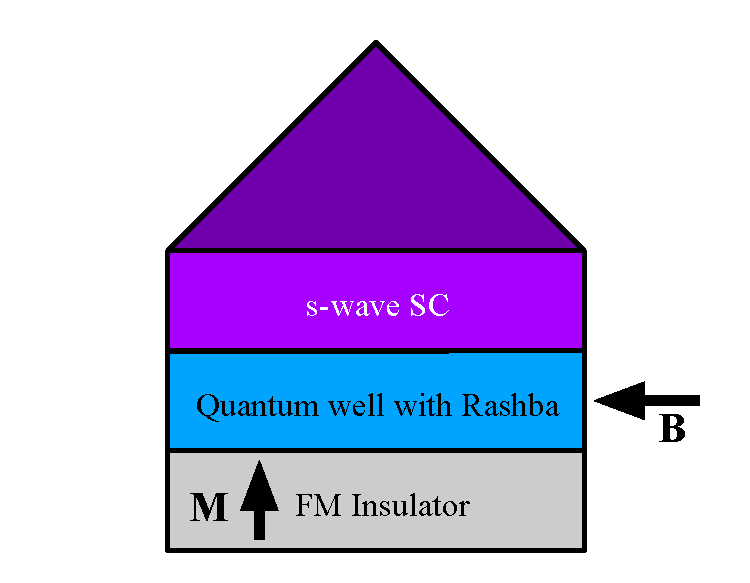
\includegraphics[width=0.5\textwidth]{./figures/tunable-semiconductor.pdf}};
        \node[inner sep=0pt] (reference) at (0,-3) {\small Alicea, \textit{PRB} \textbf{81}, 125318 (2010).};
      \end{tikzpicture}
      \small
      \begin{equation}
        c_j = (c_{j\uparrow}, c_{j\downarrow})^T
      \end{equation}
      \textit{s}-wave SC paring term:
      \begin{equation}
        \ham_{SC} = \sum_j \de \cc_{j\uparrow} \cc_{j\downarrow} + h.c.
      \end{equation}
      Quantum well:
      \begin{equation}
        \ham_0 = \sum_j (6t - \mu) \cc_j c_j - \sum_{\langle j,l \rangle} (t \cc_l c_j + h.c.)
      \end{equation}
      Rashba spin-orbit coupling:
      \begin{equation}
        \ham_R = -it_R \sum_{\langle j,l \rangle \alpha\beta} \cc_{l\alpha} (\bm{\sigma}_{\alpha\beta} \times \hat{r}_{lj}) \cdot \hat{z} c_{j\beta}
      \end{equation}
      Zeeman field:
      \begin{equation}
        \ham_Z = \sum_j \cc_j \vec{V}\cdot \bm{\sigma} c_j
      \end{equation}

    \end{multicols}
  \end{frame}

%  \begin{frame}
%    \frametitle{\PW}
%
%    \begin{figure}
%      \begin{tikzpicture}
%        %\draw[help lines,gray!20] (-4,-4) grid[step=0.5] (4,4);
%        \node[inner sep=0pt] (figure) at (-3.60,4.2)
%        {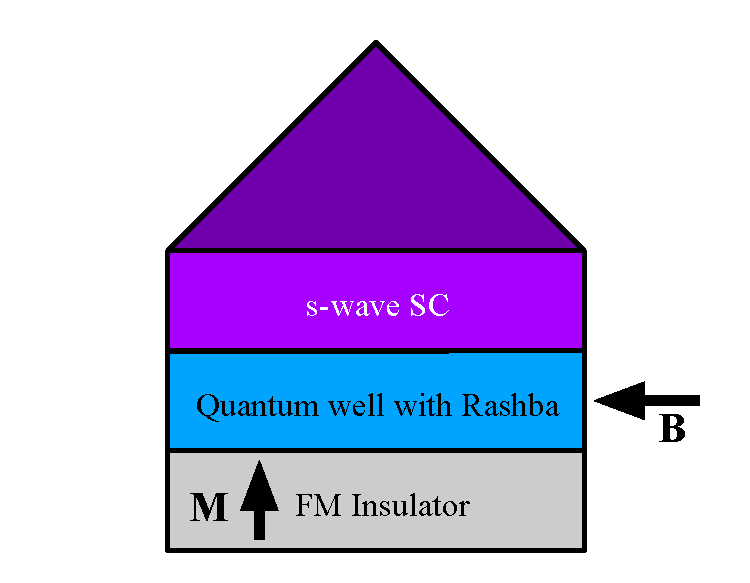
\includegraphics[width=0.35\textwidth]{./figures/tunable-semiconductor.pdf}};
%        \node[inner sep=0pt] (figure) at (2.10,4.0)
%        {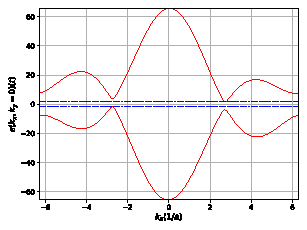
\includegraphics[width=0.40\textwidth]{./figures/dispersion-in-plane.pdf}};
%        \node[inner sep=0pt] (figure) at (-3.9,0.2)
%        {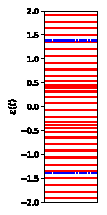
\includegraphics[width=0.14\textwidth]{./figures/energy-spectra-in-plane.pdf}};
%        \node[inner sep=0pt] (figure) at (2.5,0.2)
%        {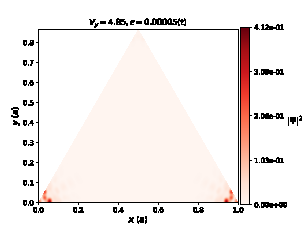
\includegraphics[width=0.40\textwidth]{./figures/wavefunction-2-in-plane.pdf}};
%        %\node[inner sep=0pt,overlay] (caption) at (-6.25,3.40) {\footnotesize$V_y = 4.85$};
%      \end{tikzpicture}
%    \end{figure}
%
%  \end{frame}

  \begin{frame}{\PW: Results}
    \begin{tikzpicture}
        \node[inner sep=0pt] (figure) at (-0.15,0.18)
        {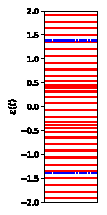
\includegraphics[width=0.16\textwidth]{./figures/energy-spectra-in-plane.pdf}};
        \node[inner sep=0pt] (figure) at (-4.0,0.0)
        {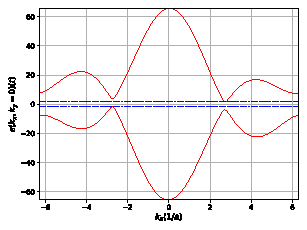
\includegraphics[width=0.45\textwidth]{./figures/dispersion-in-plane.pdf}};
        \node[inner sep=0pt] (figure) at (3.7,0.20)
        {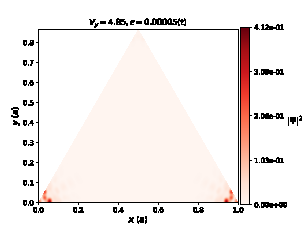
\includegraphics[width=0.45\textwidth]{./figures/wavefunction-2-in-plane.pdf}};
    \end{tikzpicture}
  \end{frame}

%  \begin{frame}{\PW}
%    \begin{tikzpicture}
%        \node[inner sep=0pt] (figure) at (-3.0,0.0)
%        {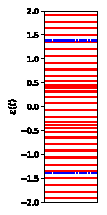
\includegraphics[width=0.30\textwidth]{./figures/energy-spectra-in-plane.pdf}};
%        \node[inner sep=0pt] (figure) at (3.2,1.9)
%        {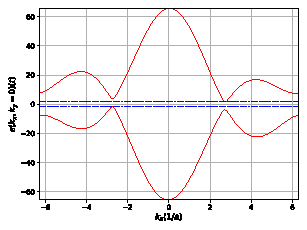
\includegraphics[width=0.40\textwidth]{./figures/dispersion-in-plane.pdf}};
%        \node[inner sep=0pt] (figure) at (3.7,-1.9)
%        {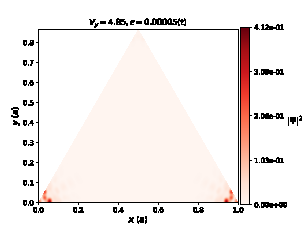
\includegraphics[width=0.40\textwidth]{./figures/wavefunction-2-in-plane.pdf}};
%    \end{tikzpicture}
%  \end{frame}

  \begin{frame}{Topological phase transition induced by a supercurrent}
    \centering
    \begin{tikzpicture}
      \node[inner sep=0pt] (figure) at (0.0,1.5)
      {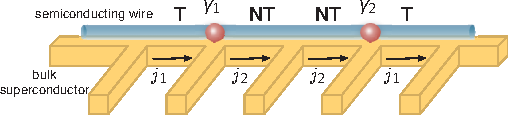
\includegraphics[width=0.6\textwidth]{./figures/Romito-setup.pdf}};
      \node[inner sep=0pt] (figure2) at (0.0,-2.0)
      {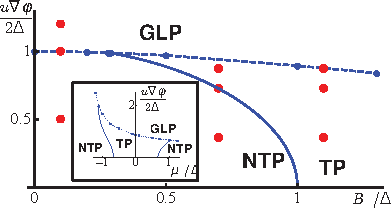
\includegraphics[width=0.6\textwidth]{./figures/Romito-topology-map2.pdf}};
      \node[inner sep=0pt] (reference) at (0,-4.5) {\small Romito et al., \textit{PRB} \textbf{85}, 020502(R) (2012).};
    \end{tikzpicture}
  \end{frame}

  \begin{frame}{Topological phase transition induced by a supercurrent}
    \centering
    \begin{tikzpicture}
      \node[inner sep=0pt] (figure) at (-3.5,0)
      {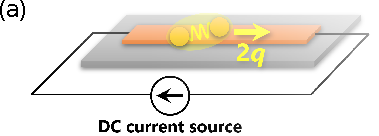
\includegraphics[width=0.4\textwidth]{./figures/Takasan-setup.pdf}};
      \node[inner sep=0pt] (figure2) at (3.0,0.0)
      {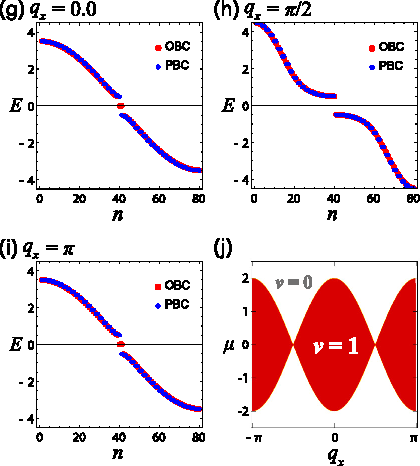
\includegraphics[width=0.5\textwidth]{./figures/Takasan-results.pdf}};
      \node[inner sep=0pt] (reference) at (-3.5,-1.5) {\small Takasan et al., \textit{PRB} \textbf{106}, 014508 (2022).};
    \end{tikzpicture}
  \end{frame}

  \begin{frame}{\FO: Two Approaches}
    \begin{itemize}
      \item Topological phase diagram for linear vector potential on Kitaev chain
      \item[] Bulk-edge correspondence for a double chain model
      \item Vector potential on a triangular island in the Kitaev limit
    \end{itemize}
  \end{frame}

  \begin{frame}{Linear vector potential and Majorana number for Kitaev chain}
    Peierls substitution
    \begin{equation}
      \vec{A} = B\vec{x}
    \end{equation}
    \begin{align}
      \cc_{j+1} c_j &\rightarrow \cc_{j+1} c_j \exp \left(-\dfrac{i e}{\hbar} \int_{r_j}^{r_{j+1}} \vec{A}(x) \cdot d\vec{l} \right) = \cc_{j+1} c_j e^{i \phi_{j+1,j}}.
    \end{align}
    \begin{equation} \label{eq: Peierls chain}
      \ham_{ch} = \sum_j (-t e^{i\phi_{j+1,j}} \cc_{j+1} c_j + \de \cc_{j+1}\cc_j + h.c.) - \mu \cc_j c_j.
    \end{equation}
    Majorana number
    \begin{equation}
      U = u \otimes I_N,\quad u = \dfrac{1}{\sqrt{2}} \left(
      \begin{matrix}
        1 & 1 \\
        -i & i
    \end{matrix} \right)
    \end{equation}
    \begin{equation}
      A_{ch} = -iU\ham_{ch}U^\dagger
    \end{equation}
    \begin{equation}
      \mathcal{M} = \text{sgn}[\text{Pf}(A_{ch})]
    \end{equation}
  \end{frame}

  \begin{frame}{Topological phase transition due to a linear vector potential}
    \begin{multicols}{2}
      \begin{tikzpicture}
        \node[inner sep=0pt] (figure) at (0,0)
        {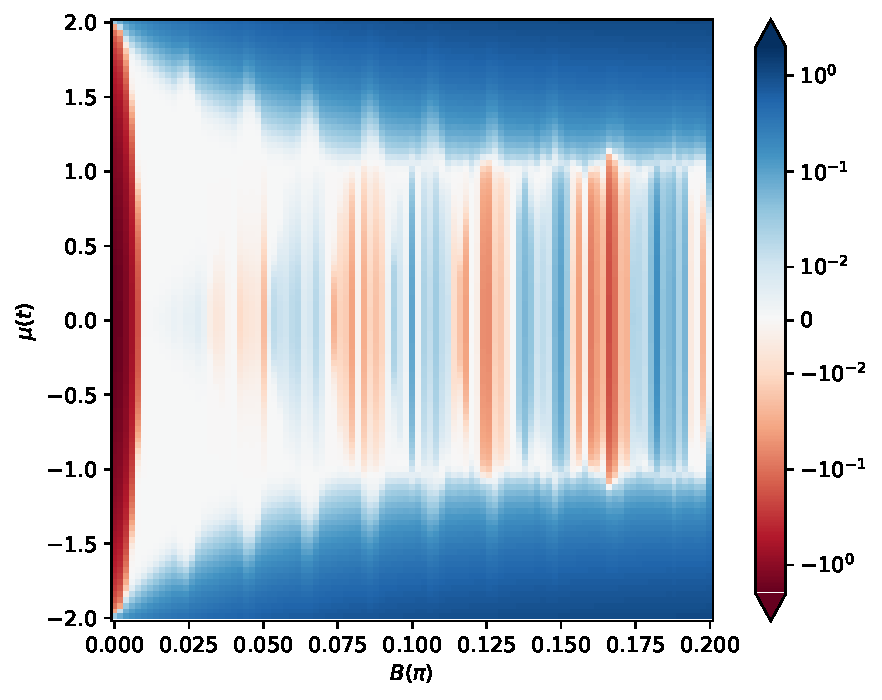
\includegraphics[width=0.5\textwidth]{./figures/linear-chain-majorana-number-full-range.pdf}};
      \end{tikzpicture}
      \vspace{10pt}
      \begin{itemize}
        \item Phase diagram shows us where the chain is (non)trivial. \\
        \pause
        \item We can use bulk-edge correspondence to force Majorana fermions at the interface between differing topologies with large enough gaps. \\
        \item Double chain toy model:
      \end{itemize}
      \vspace{10pt}
      \begin{tikzpicture}
        \node[inner sep=0pt] (figure) at (0,0)
        {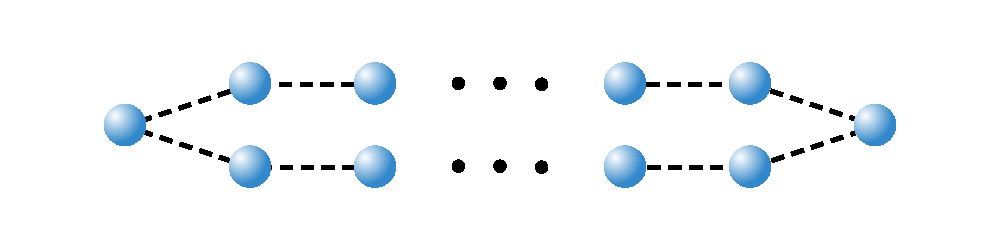
\includegraphics[width=0.5\textwidth]{./figures/double-chain.pdf}};
        \node[inner sep=0pt] (Aon) at (0,0.8) {\small $\vec{A} = B\vec{x}$};
        \node[inner sep=0pt] (Aoff) at (0,-0.8) {\small $\vec{A} = 0$};
      \end{tikzpicture}
    \end{multicols}
  \end{frame}

  \begin{frame}{Bulk-edge correspondence on a double chain}
    \centering
    \begin{tikzpicture}
      \node[inner sep=0pt] (figure) at (0,4)
      {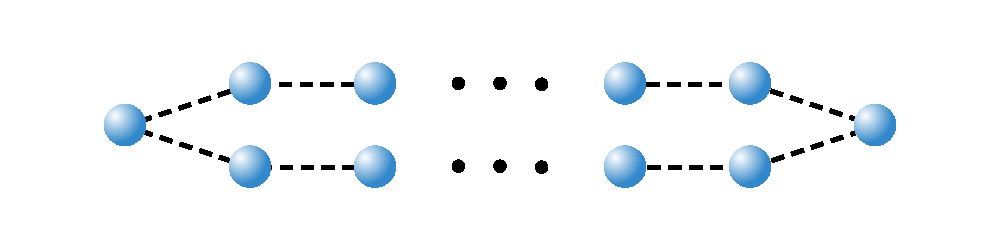
\includegraphics[width=0.5\textwidth]{./figures/double-chain.pdf}};
      \node[inner sep=0pt] (Aon) at (0,4.8) {\small $\vec{A} = 0.16\pi\vec{x}$};
      \node[inner sep=0pt] (Aoff) at (0,3.2) {\small $\vec{A} = 0$};
      \node[inner sep=0pt] (figure) at (-4.8,3.85)
      {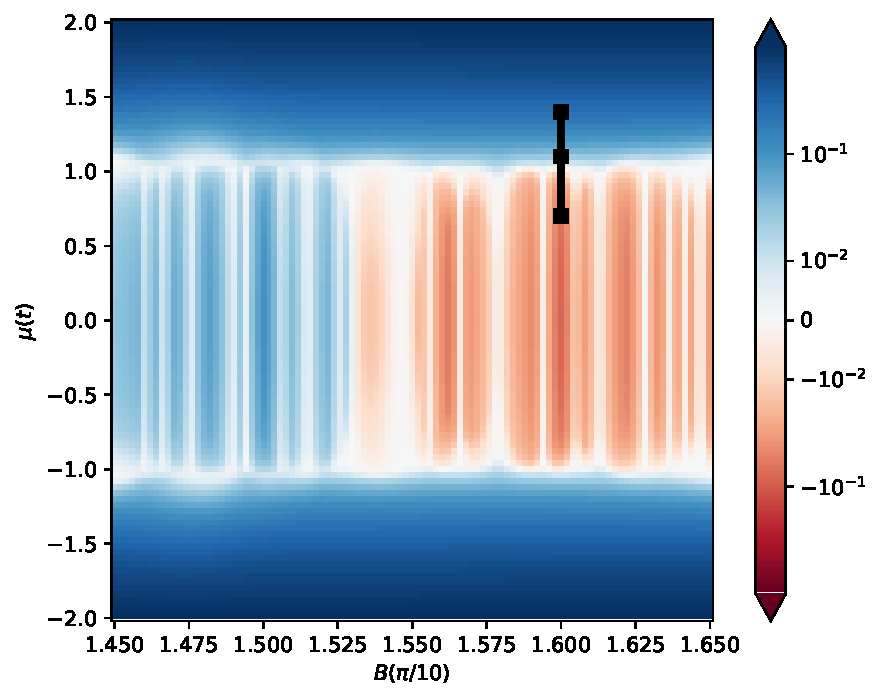
\includegraphics[width=0.30\textwidth]{./figures/linear-chain-majorana-number-B-1_6.pdf}};
      \node[inner sep=0pt] (figure) at (-4.5,0)
      {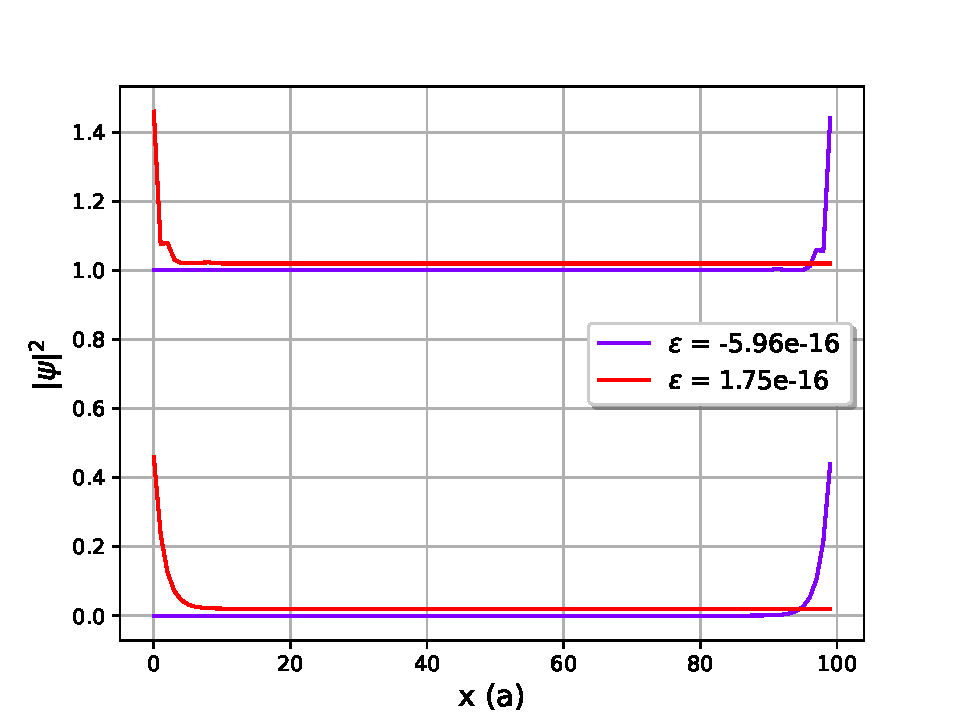
\includegraphics[width=0.38\textwidth]{./figures/double-chain-mu-p1_4-B-0_16pi.pdf}};
      \node[inner sep=0pt] (mu1) at (-4.5,1.7) {\small $\mu = 1.4t$};
      \pause
      \node[inner sep=0pt] (figure) at (0,0)
      {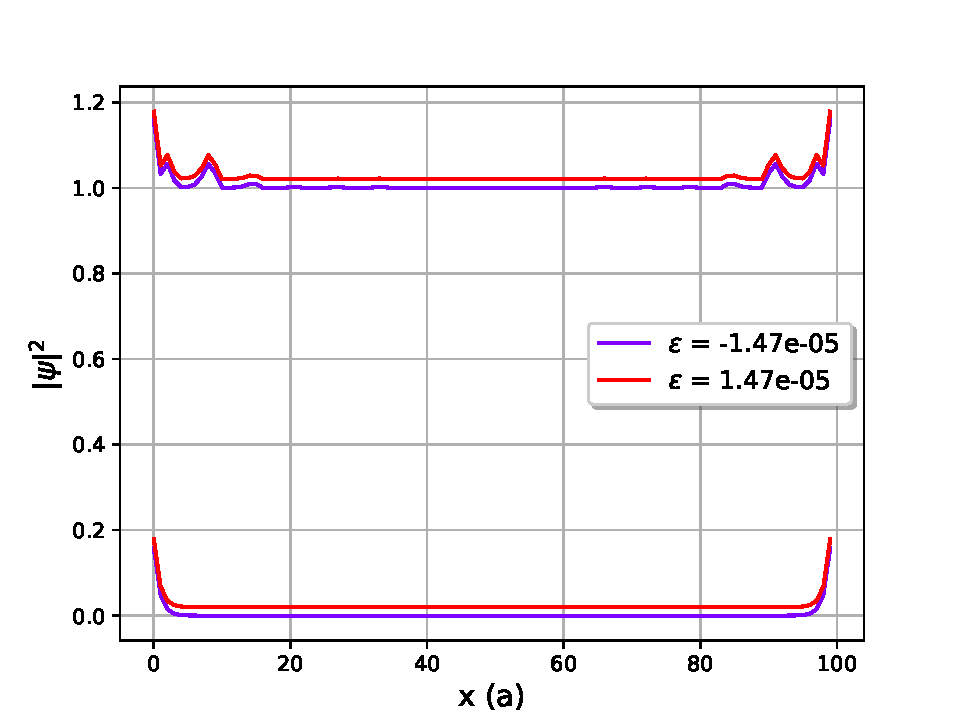
\includegraphics[width=0.38\textwidth]{./figures/double-chain-mu-p1_1-B-0_16pi.pdf}};
      \node[inner sep=0pt] (mu2) at (0,1.7) {\small $\mu = 1.1t$};
      \pause
      \node[inner sep=0pt] (figure) at (4.5,0)
      {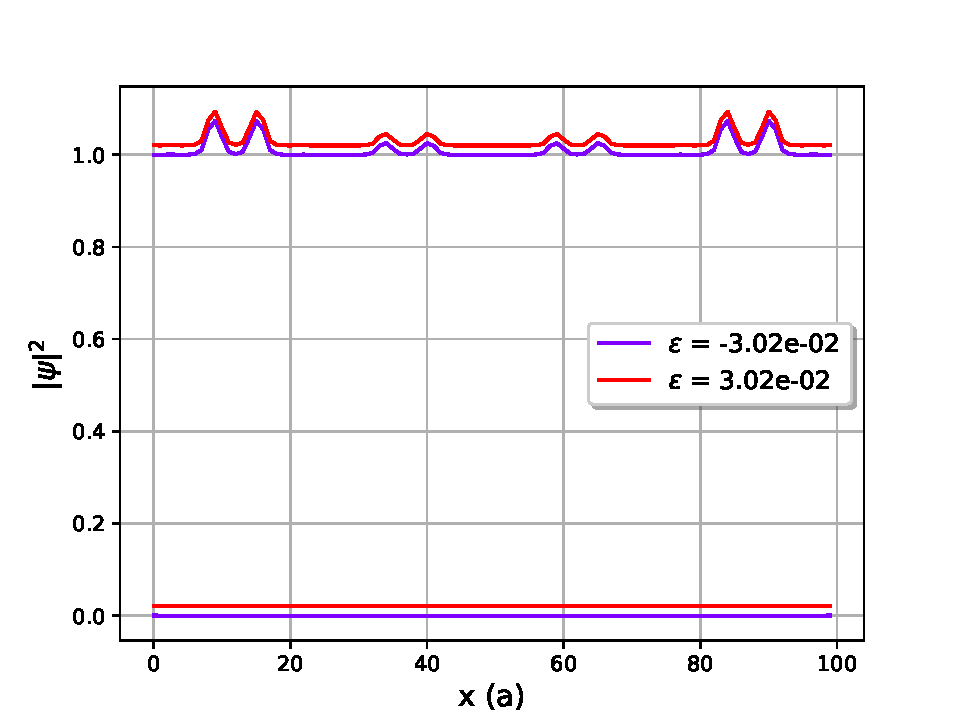
\includegraphics[width=0.38\textwidth]{./figures/double-chain-mu-p0_7-B-0_16pi.pdf}};
      \node[inner sep=0pt] (mu3) at (4.5,1.7) {\small $\mu = 0.7t$};
    \end{tikzpicture}
  \end{frame}

  \begin{frame}{Bulk-edge correspondence on a double chain}
    \centering
    \begin{tikzpicture}
      \node[inner sep=0pt] (figure) at (0,4)
      {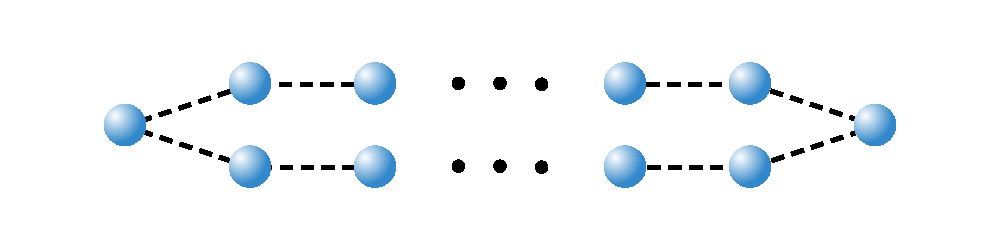
\includegraphics[width=0.5\textwidth]{./figures/double-chain.pdf}};
      \node[inner sep=0pt] (Aon) at (0,4.8) {\small $\vec{A} = 0.15\pi\vec{x}$};
      \node[inner sep=0pt] (Aoff) at (0,3.2) {\small $\vec{A} = 0$};
      \node[inner sep=0pt] (figure) at (-4.8,3.85)
      {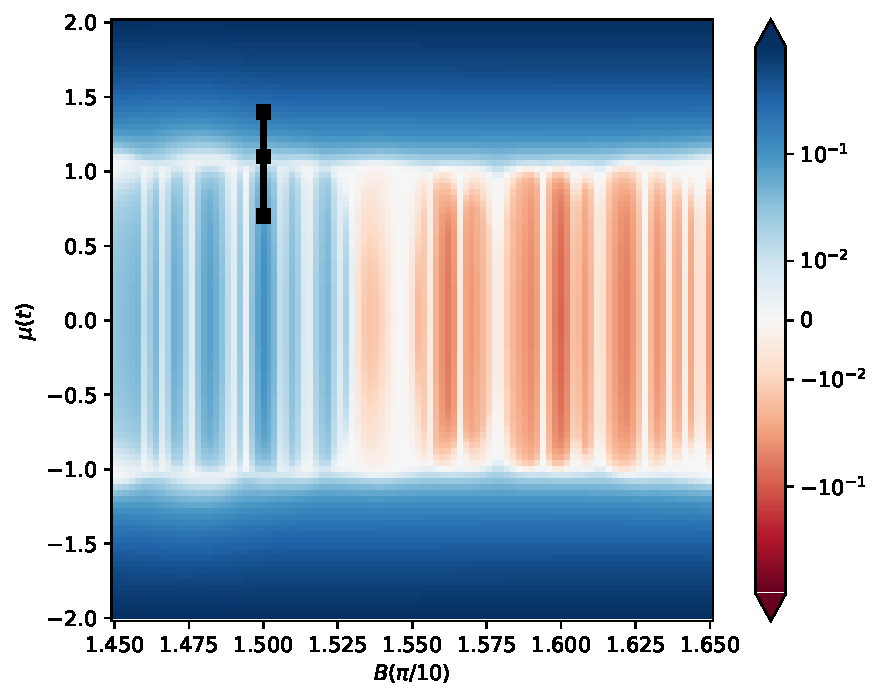
\includegraphics[width=0.30\textwidth]{./figures/linear-chain-majorana-number-B-1_5.pdf}};
      \node[inner sep=0pt] (figure) at (-4.5,0)
      {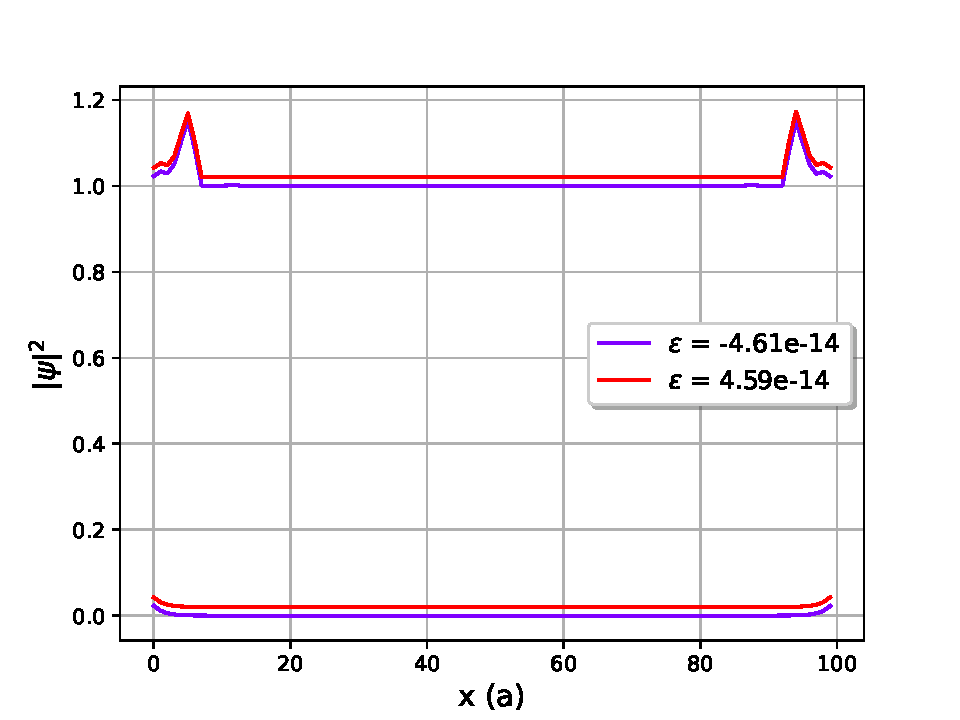
\includegraphics[width=0.38\textwidth]{./figures/double-chain-mu-p1_4-B-0_15pi.pdf}};
      \node[inner sep=0pt] (mu1) at (-4.5,1.7) {\small $\mu = 1.4t$};
      \pause
      \node[inner sep=0pt] (figure) at (0,0)
      {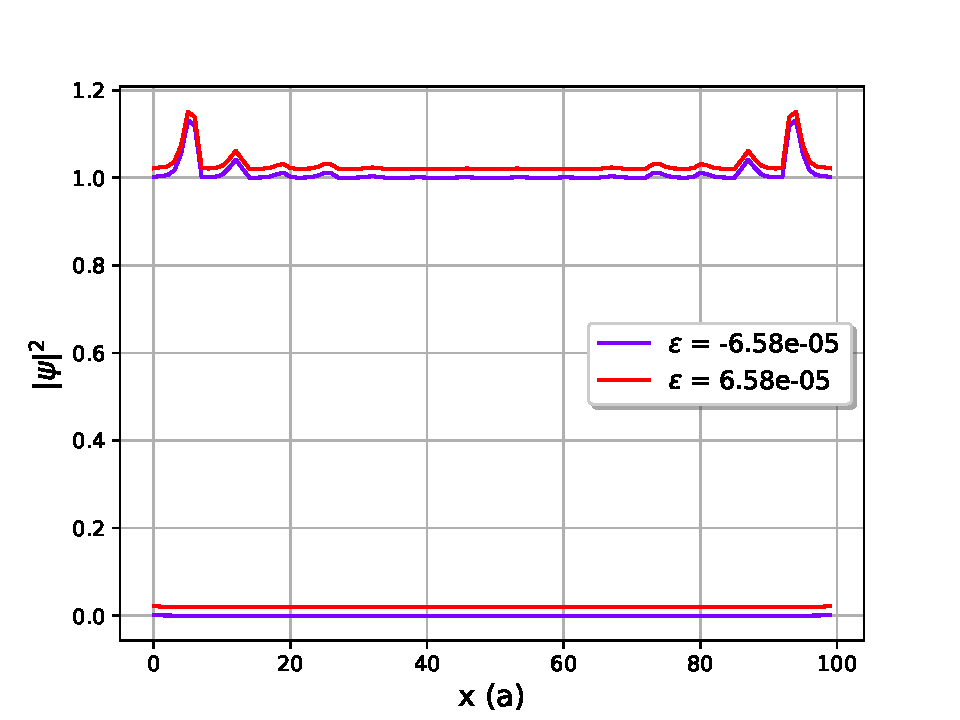
\includegraphics[width=0.38\textwidth]{./figures/double-chain-mu-p1_1-B-0_15pi.pdf}};
      \node[inner sep=0pt] (mu1) at (0,1.7) {\small $\mu = 1.1t$};
      \pause
      \node[inner sep=0pt] (figure) at (4.5,0)
      {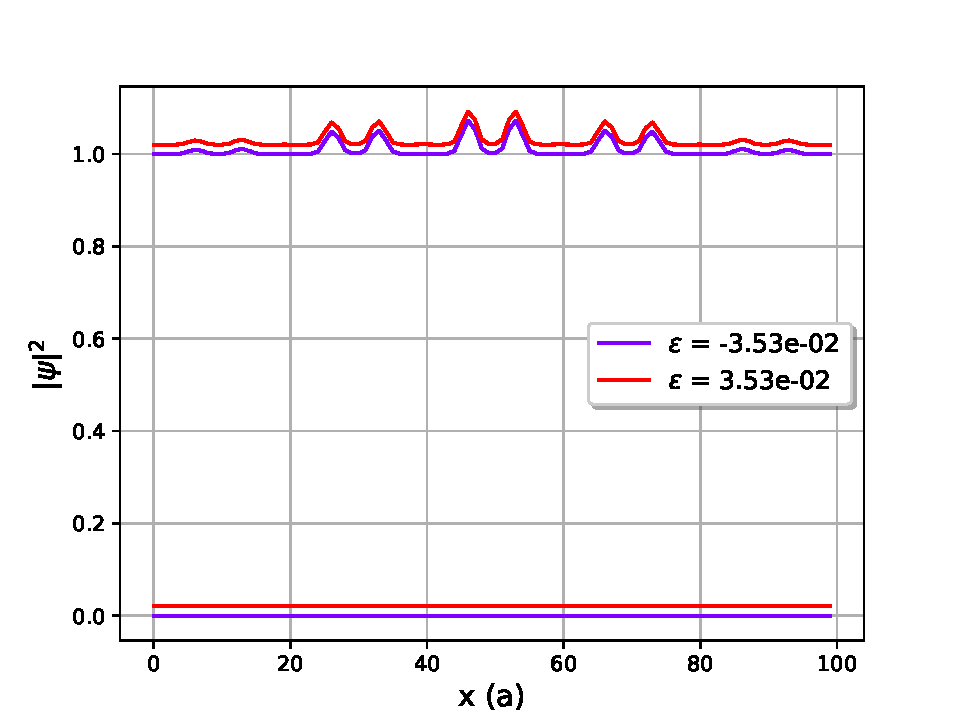
\includegraphics[width=0.38\textwidth]{./figures/double-chain-mu-p0_7-B-0_15pi.pdf}};
      \node[inner sep=0pt] (mu3) at (4.5,1.7) {\small $\mu = 0.7t$};
    \end{tikzpicture}
  \end{frame}

%  \begin{frame}
%    \frametitle{Kitaev Limit with Vector Potential on a Triangular Island}
%
%    \begin{multicols}{2}
%    % show condition for there to be a MF at one corner and show a picture
%      \begin{tikzpicture}
%        %\draw[help lines,gray!20] (-4,-4) grid[step=0.5] (4,4);
%        \node[inner sep=0pt] (figure) at (0,0)
%        {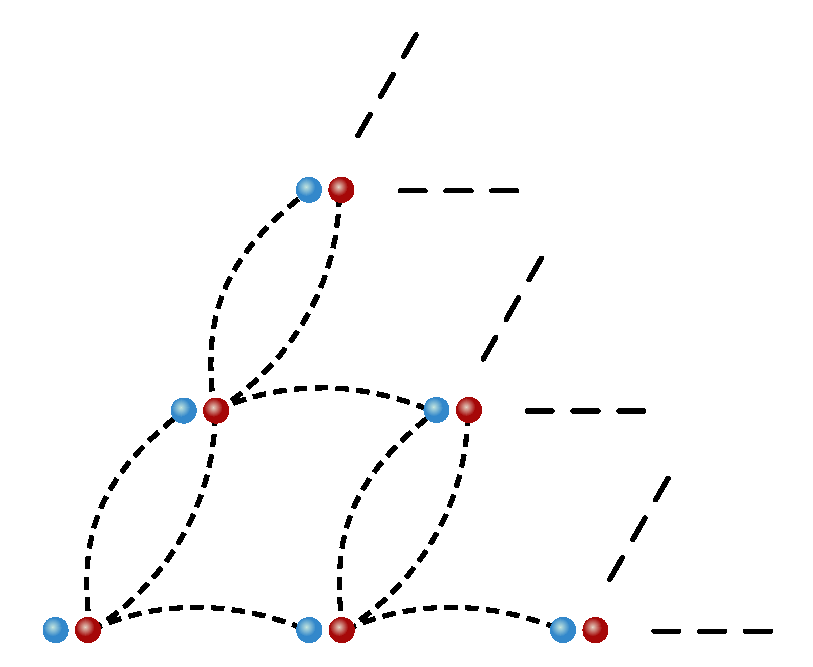
\includegraphics[width=.4\textwidth]{./figures/left-triangle-corner.pdf}};
%      \end{tikzpicture}
%
%      \small
%      \begin{gather*}
%        \hspace{-5em}
%        \ham = \sum_{<j,l>} \left[ -t e^{i\phi_{l,j}}\cc_{l} c_j + \de e^{i\theta_{l,j}} \cc_{l}\cc_j + h.c.\right] - \sum_j \mu \cc_j c_j \\
%        \hspace{-5em}
%        \phi_{l,j} = -\dfrac{e}{\hbar}\int_{\vec{r}_j}^{\vec{r}_l} \vec{A} \cdot d\vec{l} \\
%        \hspace{-5em}
%        \vec{A} = -\dfrac{2 \pi}{3\sqrt{3} a} \hat{y}\\
%        \hspace{-5em}
%        t = \de, \ \mu=0
%      \end{gather*}
%      \vspace{20em}
%
%    \end{multicols}
%
%  \end{frame}

  \begin{frame}{Triangular \textit{p}-wave superconductor with vector potential}
    \textit{p}-wave superconductor Hamiltonian with vector potential
    \begin{equation}
      \ham = \sum_{\langle j,l \rangle} \left[ -t e^{i\phi_{l,j}}\cc_{l} c_j + \de e^{i\theta_{l,j}} \cc_{l}\cc_j + h.c.\right] - \sum_j \mu \cc_j c_j,
    \end{equation}
    where
    \begin{equation}
      \phi_{l,j} = -\dfrac{ie}{\hbar} \int_{\vec{r}_j}^{\vec{r}_l} \vec{A}(x) \cdot d\vec{l}.
    \end{equation}
    \textit{p}-wave superconductor Hamiltonian in Majorana fermion basis
    \begin{align}
      \ham = -\dfrac{i\mu}{4} \sum_j (& a_j b_j - b_j a_j) \nonumber \\
      -\dfrac{i}{2} \sum_{\langle j,l\rangle} [&(t\sin\phi_{l.j}-\de\sin\theta_{l,j}) a_l a_j
      +(t\sin\phi_{l,j}+\de\sin\theta_{l,j}) b_l b_j \nonumber \\
      +&(t\cos\phi_{l,j}+\de\cos\theta_{l,j}) a_l b_j
      -(t\cos\phi_{l,j}-\de\cos\theta_{l,j}) b_l a_j].
    \end{align}

  \end{frame}

  \begin{frame}{Conditions for MZMs on a triangular island}
    \begin{minipage}{\textwidth}
    \begin{multicols}{2}
    Start with Kitaev limit $t = \de \neq 0$ and $\mu=0$.
    \begin{align}
      &t (\sin\phi_{l,j} - \sin\theta_{l,j}) a_l a_j, \\
      &t (\sin\phi_{l,j} + \sin\theta_{l,j}) b_l b_j, \\
      &t (\cos\phi_{l,j} + \cos\theta_{l,j}) a_l b_j, \\
      &t (\cos\phi_{l,j} - \cos\theta_{l,j}) b_l a_j
    \end{align}
    \centering
    \begin{tikzpicture}
      \node[inner sep=0pt] (figure) at (0,0)
      {\includegraphics[width=0.35\textwidth]{./figures/3-point-triangle.pdf}};
      \node[inner sep=0pt] (a1) at (-1.45,-1.6) {\small $a_1$ \ $b_1$};
      \node[inner sep=0pt] (a2) at (1.5,-1.6) {\small $a_2$ \ $b_2$};
      \node[inner sep=0pt] (a3) at (0.0,1.65) {\small $a_3$ \ $b_3$};
    \end{tikzpicture}
    \end{multicols}
    \vspace{2pt}
    \end{minipage}
    \begin{itemize}
      \item Need $a_3 a_1$, $b_3 a_1$, $b_2 a_3$ and $b_2 b_3$ to have zero weight. \\
      \item We find $\phi_{3,1} = \pi/3$ and $\phi_{2,3}=\pi/3$. \\
      \item This critical condition is met for odd function vector potentials. For a linear vector potential:
    \end{itemize}
    \begin{equation}
      \vec{A}_0(x) = \dfrac{8\pi}{3\sqrt{3}a^2} x \hat{y} = B_0 x \hat{y}.
    \end{equation}
  \end{frame}

  \section{\RE}

  \begin{frame}{Triangular island}
    \begin{multicols}{2}
      Extrapolate the critical vector strength from a 3-point triangle to a triangle with $n_r$ rows.\\
      \begin{align}
        B_0 &= \dfrac{8\pi}{3\sqrt{3}a^2} \dfrac{1}{2n_r - 3} \\
        \vec{A} &= B x \hat{y} \nonumber
      \end{align}
      \centering
      \begin{figure}
        \includegraphics[width=0.35\textwidth]{./figures/vector-potential-field.pdf}
      \end{figure}
      \vspace{10pt}
      \begin{tikzpicture}
        \node[inner sep=0pt] (figure1) at (0,2)
        {\includegraphics[width=0.37\textwidth]{../../../research-code/mf-quantum-logic-gate-scripts/data/figures/linear-vector-potential/nr-25/w-0/mu-p0_0000/spectral-flow.pdf}};
        \node[inner sep=0pt] (figure2) at (0,-1.7)
        {\includegraphics[width=0.37\textwidth]{../../../research-code/mf-quantum-logic-gate-scripts/data/figures/linear-vector-potential/nr-25/w-0/mu-p0_0000/En00-B-0_1029.pdf}};
      \end{tikzpicture}
      \vspace{10pt}

    \end{multicols}
  \end{frame}

  \begin{frame}
    \frametitle{Triangular Chain}
    % show spectral plot and wavefunction
    \begin{tikzpicture}
      \node[inner sep=0pt] (figure) at (-3.2,0)
      {\includegraphics[width=0.5\textwidth]{../../../research-code/mf-quantum-logic-gate-scripts/data/figures/linear-vector-potential/nr-25/w-1/mu-p0_0000/spectral-flow.pdf}};
      \node[inner sep=0pt] (figure) at (3.2,-0.15)
      {\includegraphics[width=0.5\textwidth]{../../../research-code/mf-quantum-logic-gate-scripts/data/figures/linear-vector-potential/nr-25/w-1/mu-p0_0000/Ep00-B-0_1029.pdf}};
    \end{tikzpicture}

  \end{frame}

  \begin{frame}
    \frametitle{Hollow Triangle}

    \begin{figure}
      \begin{tikzpicture}
        \node[inner sep=0pt] (figure) at (-3.2,0)
        {\includegraphics[width=0.5\textwidth]{../../../research-code/mf-quantum-logic-gate-scripts/data/figures/linear-vector-potential/nr-25/w-3/mu-p0_0000/spectral-flow.pdf}};
        \node[inner sep=0pt] (figure) at (3.2,-0.15)
        {\includegraphics[width=0.5\textwidth]{../../../research-code/mf-quantum-logic-gate-scripts/data/figures/linear-vector-potential/nr-25/w-3/mu-p0_0000/En00-B-0_1029.pdf}};
      \end{tikzpicture}
    \end{figure}
  \end{frame}

  \section{\CO}
  \begin{frame}
    \frametitle{\CO}

    \begin{itemize}
      \item Triangular islands with a gapped interior can be a promising platform for hosting and manipulating MZMs.
      \item Next steps
      \begin{itemize}
        \item Search for robust MZMs in hollow triangles outside the Kitaev limit using a Topological phase diagram.
        \item Reapply the methodology for a Rashba SC heterostructure.
        \item Develop a practical braiding scheme.
      \end{itemize}
    \end{itemize}
    \centering
    \begin{tikzpicture}
      \node[inner sep=0pt] (figure) at (-3,0)
      {\includegraphics[width=0.4\textwidth]{./figures/linear-chain-majorana-number-full-range.pdf}};
      \node[inner sep=0pt] (figure) at (3,0)
      {\includegraphics[width=0.45\textwidth]{../../../research-code/mf-quantum-logic-gate-scripts/data/figures/linear-vector-potential/nr-25/w-3/mu-p0_0000/En00-B-0_1029.pdf}};
    \end{tikzpicture}
  \end{frame}

  \begin{frame}{Additional projects}

    \begin{itemize}
      \item Using a semi-infinite tight binding model to find Floquet Landau levels for Graphene and 2DEGs using two linearly polarized lights.
      \item Kitaev mapped spins to fermions using the Jordan-Wigner transformation. Can we achieve similar results using one of our triangular structures?
    \end{itemize}
  \end{frame}

  \appendix

  \begin{frame}
    \frametitle{Additional results from Schneider et al.}

    \begin{figure}
      \includegraphics[width=0.8\textwidth]{./figures/Schneider-additional-results.pdf}
    \end{figure}

  \end{frame}

  \begin{frame}
  \frametitle{Majorana fermion notation and coupling isolations}
    The complex fermion operator can be written as a superposition of two Majorana fermions $c_j = \frac{1}{2} (a_j + i b_j)$.
    Due to the nature of Majorana fermions, $a^{\dagger}_j = a_j$, the creation operator is $\cc_j = \frac{1}{2} (a_j - i b_j)$.
    \begin{align*}
      H = -\dfrac{i\mu}{4} \sum_j (a_j b_j - b_j a_j) - \dfrac{i}{4} \sum_{<j,l>} [&(t\sin\phi-\de\sin\theta) a_l a_j + (t\sin\phi+\de\sin\theta) b_l b_j \nonumber \\
      +&(t\cos\phi+\de\cos\theta) a_l b_j - (t\cos\phi-\de\cos\theta) b_l a_j].
    \end{align*}
    \begin{align}
      &(t \sin\phi_{j,l} - \de \sin\theta_{j,l}) a_l a_j, \\
      &(t \sin\phi_{j,l} + \de \sin\theta_{j,l}) b_l b_j, \\
      &(t \cos\phi_{j,l} + \de \cos\theta_{j,l}) a_l b_j, \\
      &(t \cos\phi_{j,l} - \de \cos\theta_{j,l}) b_l a_j
    \end{align}
  \end{frame}

  \begin{frame}
    \frametitle{Triangular chain degeneracy}

    \begin{figure}
      \includegraphics[width=0.8\textwidth]{../../../research-code/mf-quantum-logic-gate-scripts/data/figures/linear-vector-potential/nr-25/w-1/mu-p0_0000/En00-B-0_1029.pdf}
    \end{figure}

  \end{frame}

  \begin{frame}
    \frametitle{Hollow triangle degeneracy?}

    \begin{figure}
      \includegraphics[width=0.8\textwidth]{../../../research-code/mf-quantum-logic-gate-scripts/data/figures/linear-vector-potential/nr-25/w-3/mu-p0_0000/En01-B-0_1029.pdf}
    \end{figure}

  \end{frame}


\end{document}


